%% Copernicus Publications Manuscript Preparation Template for LaTeX Submissions
%% ---------------------------------
%% This template should be used for copernicus.cls
%% The class file and some style files are bundled in the Copernicus Latex Package, which can be downloaded from the different journal webpages.
%% For further assistance please contact Copernicus Publications at: production@copernicus.org
%% https://publications.copernicus.org/for_authors/manuscript_preparation.html


%% Please use the following documentclass and journal abbreviations for discussion papers and final revised papers.

%% 2-column papers and discussion papers
\documentclass[journal abbreviation, manuscript]{copernicus}



%% Journal abbreviations (please use the same for discussion papers and final revised papers)


% Advances in Geosciences (adgeo)
% Advances in Radio Science (ars)
% Advances in Science and Research (asr)
% Advances in Statistical Climatology, Meteorology and Oceanography (ascmo)
% Annales Geophysicae (angeo)
% Archives Animal Breeding (aab)
% ASTRA Proceedings (ap)
% Atmospheric Chemistry and Physics (acp)
% Atmospheric Measurement Techniques (amt)
% Biogeosciences (bg)
% Climate of the Past (cp)
% DEUQUA Special Publications (deuquasp)
% Drinking Water Engineering and Science (dwes)
% Earth Surface Dynamics (esurf)
% Earth System Dynamics (esd)
% Earth System Science Data (essd)
% E&G Quaternary Science Journal (egqsj)
% European Journal of Mineralogy (ejm)
% Fossil Record (fr)
% Geochronology (gchron)
% Geographica Helvetica (gh)
% Geoscience Communication (gc)
% Geoscientific Instrumentation, Methods and Data Systems (gi)
% Geoscientific Model Development (gmd)
% History of Geo- and Space Sciences (hgss)
% Hydrology and Earth System Sciences (hess)
% Journal of Micropalaeontology (jm)
% Journal of Sensors and Sensor Systems (jsss)
% Mechanical Sciences (ms)
% Natural Hazards and Earth System Sciences (nhess)
% Nonlinear Processes in Geophysics (npg)
% Ocean Science (os)
% Primate Biology (pb)
% Proceedings of the International Association of Hydrological Sciences (piahs)
% Scientific Drilling (sd)
% SOIL (soil)
% Solid Earth (se)
% The Cryosphere (tc)
% Weather and Climate Dynamics (wcd)
% Web Ecology (we)
% Wind Energy Science (wes)


%% \usepackage commands included in the copernicus.cls:
%\usepackage[german, english]{babel}
\usepackage{tabularx}
%\usepackage{cancel}
\usepackage{multirow}
%\usepackage{supertabular}
%\usepackage{algorithmic}
%\usepackage{algorithm}
%\usepackage{amsthm}
%\usepackage{float}
%\usepackage{subfig}
%\usepackage{rotating}

\usepackage{booktabs}

\begin{document}

\title{Do the  climate (AeroCom phase III / CMIP6) models reproduce the observed aerosol trends over the last two decades?}

% \Author[affil]{given_name}{surname}
\Author[1]{Augustin}{Mortier}
\Author[1]{Jonas}{Gliss}
\Author[1]{Michael}{Schulz}
\Author[2]{others}{}
\affil[1]{Norwegian Meteorological Institute}
\affil[2]{ADDRESS}

%% The [] brackets identify the author with the corresponding affiliation. 1, 2, 3, etc. should be inserted.
%% If an author is deceased, please add a further affiliation and mark the respective author name(s) with a dagger, e.g. "\Author[2,$\dag$]{Anton}{Aman}" with the affiliations "\affil[2]{University of ...}" and "\affil[$\dag$]{deceased, 1 July 2019}"


\correspondence{Mortier (augustinm@met.no)}

\runningtitle{Aerosol Trends}

\runningauthor{Augustin Mortier}

\received{}
\pubdiscuss{} %% only important for two-stage journals
\revised{}
\accepted{}
\published{}
%% These dates will be inserted by Copernicus Publications during the typesetting process.


\firstpage{1}

\maketitle

%\tableofcontents

\begin{abstract}
 TEXT
\end{abstract}


\copyrightstatement{TEXT}


\introduction  %% \introduction[modified heading if necessary]
TEXT
\begin{itemize}
 \item importance of aerosols for health, climate..
 \item aerosols uncertainty due to high variability in space and time at different scales
 \item in addition to seasonal variability, variability at a longer time-scale. Importance of assessing the aerosol trends.
 \item sources of variability: anthropogenic emissions (development of emergent countries VS mitigation measures: e.g: Clean Air Act), changes in meteorological conditions that parameterize the emissions of natural aerosols and the wet and dry deposition of aerosols.
 \item the ground based observation of the aerosols is organized in different networks. The remote sensing networks provide optical properties of the aerosols in the total air column, while in situ measurements provide particles measurements at the surface level. Using both of these information allow to depict a more complete picture of the changes in the aerosol content.
 \item what do the aerosol trends look like as seen from these observation networks?
 \item because of the role of aerosol on climate, it is of importance for the models to capture the aerosol trends in order to reproduce the climate trends. How do the models reproduce the aerosol trends?
 \item can we use models to assess the global aerosol trends?
 \item in regards of the availability of the data used in this study, start in 2000. Last year of CMIP6 historical runs: 2000 -> study period: 2000-2014.
\end{itemize}


\section{Datasets}
A set of nine optical and in situ aerosol measurements is used in this study. The observation networks and the models providing output for these parameters are reported in Table \ref{table:datasets}.

\begin{table}
 \begin{tabularx}{\textwidth}{lllX}
  \tophline
  Parameter   & Type    & Observation network & Models                                                                                                    \\
  \middlehline
  AOD         & Column  & AERONET             & ECMWF-Rean; NorESM2; SPRINTARS; ECHAM-HAM; GEOS; OsloCTM3; GFDL-AM4; BCC-CUACE; CanESM5; CESM2; IPSL-CM6A \\
  AOD<1µm     & Column  & AERONET             & NorESM2; SPRINTARS; ECHAM-HAM; GEOS; GFDL-AM4                                                             \\
  AOD>1µm     & Column  & AERONET             & ECMWF-Rean; NorESM2; SPRINTARS; ECHAM-HAM; OsloCTM3; GFDL-AM4; BCC-CUACE                                  \\
  AE          & Column  & AERONET             & ECMWF-Rean; NorESM2; SPRINTARS; ECHAM-HAM; GEOS; OsloCTM3; GFDL-AM4                                       \\
  $PM_{2.5}$  & Surface & GAW                 & ECMWF-Rean; NorESM2                                                                                       \\
  $PM_{10}$   & Surface & GAW                 & ECMWF-Rean; NorESM2; SPRINTARS; ECHAM-HAM; GEOS                                                           \\
  $SO_{4}$    & Surface & GAW/TAD             & ECMWF-Rean; NorESM2; SPRINTARS; ECHAM-HAM; GEOS; OsloCTM3; BCC-CUACE                                      \\
  Scat. Coef. & Surface & GAW/IMPROVE/ACTRIS  & NorESM2                                                                                                   \\
  Abs. Coef.  & Surface & GAW/IMPROVE/ACTRIS  & NorESM2; SPRINTARS                                                                                        \\
  \bottomhline
 \end{tabularx}
 \caption{List of observation and model datasets used in this study.}
 \label{table:datasets}
\end{table}

\subsection{Observations}

We use the highest quality level available, apply non-validity flags and an outliers range (see corresponding bullet-point).

\subsubsection{Sunphotometer}
(AERONET website): The AERONET (AErosol RObotic NETwork) project is a federation of ground-based remote sensing aerosol networks established by NASA and PHOTONS (PHOtométrie pour le Traitement Opérationnel de Normalisation Satellitaire; Univ. of Lille 1, CNES, and CNRS-INSU) and is greatly expanded by networks (e.g., RIMA, AeroSpan, AEROCAN, and CARSNET) and collaborators from national agencies, institutes, universities, individual scientists, and partners. For more than 25 years, the project has provided long-term, continuous and readily accessible public domain database of aerosol optical, microphysical and radiative properties for aerosol research and characterization, validation of satellite retrievals, and synergism with other databases. The network imposes standardization of instruments, calibration, processing and distribution.


** USED IN THIS STUDY AERONET: level2.0 (quality assured), version 3** + daily files

\begin{itemize}
 \item Sun Direct measurements
       \begin{itemize}
        \item AOD (Aerosol Optical Depth).
        \item AE (Anstrom Exponent): calculated using 440 nm and 870 nm channels.
       \end{itemize}
 \item Spectral Deconvolution Algorithm (SDA, described in \cite{o2003spectral})
       \begin{itemize}
        \item AOD<1µm (AOD for the particles whose diameter is lower than 1 µm).
        \item AOD>1µm (AOD for the particles whose diameter is greater than 1 µm).
       \end{itemize}
\end{itemize}


All the following data have been downloaded via EBAS platform (\cite{ebasweb}).
(EBAS website): EBAS is a database hosting observation data of atmospheric chemical composition and physical properties. EBAS hosts data submitted by data originators in support of a number of national and international programs ranging from monitoring activities to research projects. EBAS is developed and operated by the Norwegian Institute for Air Research (NILU).

\subsubsection{Particule Matter}
GAW (GAW website): The Global Atmosphere Watch (GAW) programme of WMO is a partnership involving the Members of WMO, contributing networks and collaborating organizations and bodies which provides reliable scientific data and information on the chemical composition of the atmosphere, its natural and anthropogenic change, and helps to improve the understanding of interactions between the atmosphere, the oceans and the biosphere.
*In North America, data only until 2006*
\begin{itemize}
 \item $PM_{10}$ (\unit{µg.m^{-3}})
 \item $PM_{2.5}$ (\unit{µg.m^{-3}})
\end{itemize}

\subsubsection{$SO_{4}$ concentration}
(trends website): The global dataset is prepared by the WMO/GAW Science Advisory Group for Total Atmospheric Deposition (SAG-TAD) based on data from different regional and global networks:
\begin{itemize}
 \item WMO/GAW: World Data Center for Precipitation Chemistry
 \item CASTNET: Clean Air Status and Trends Network
 \item NADP: National Atmospheric Deposition Program
 \item CAPMoN: The Canadian Air and Precipitation Monitoring Network
 \item EMEP: The European Monitoring and Evaluation Program
 \item IDAF/DEBITS: Atmospheric Chemistry Monitoring Network in Africa / DEposition of Biogeochemically Important Trace Species
 \item EANET: Acid Deposition Network in East Asia
\end{itemize}

Subset from Aas et al.
The data has been screened to be regional representative and of satisfactory quality:
Precipitation measurements are mainly from wet-only samplers or bulk if proven comparable to wet-only.
The sampling frequency is 2 weeks or higher –mostly daily measurements, except African data where precipitation is sampled on rain events and SO2 with monthly passive samplers.
Wet deposition and volume weighted precipitation data are based are based on the standard rain gauge depth if that is measured in parallel. At other sites without rain gauge, the sample depth are used.
Urban sites are not included, neither sites where the surroundings have changed considerable in the period in question.
When averaging monthly data with higher sampling frequency than daily, the sample is weighted in accordance to how many days it has been sampled in that month.

\subsubsection{Optical in situ}
\begin{itemize}
 \item Scattering coefficient (\unit{Mm^{-1}}): from nephelometer - dry -> RH<30\%? - Validity range: [-10,1000]
 \item Absorption coefficients (\unit{Mm^{-1}}): from aethalometer - validity range: [-1,100] - Removed Alert station (unit issue).
\end{itemize}

\subsection{Models}
**Describe model groups**
A set of 11 climate models are used in this study. Their main characteristics are reported in Table \ref{table:models}.  One can separate them into three groups.

\subsubsection{CAMS-Reanalysis}
w. data assimilation

\subsubsection{AeroCom phase III}
historical runs.
required output: + additional output for some models, which permits to cover the nine aerosol parameters.
Also, nudged / not-nudged AP3?

\subsubsection{CMIP6}
required output: od550aer time series from xxxx to 2014.

\begin{table}
 \begin{tabularx}{\textwidth}{lllllX}
  \tophline
  Model      & Group     & Emission & Meteorology & LatxLon resolution (degree) & References                                                          \\
  \middlehline
  ECMWF-Rean & CAMS-Rean & ?        & ?           & 1.12x1.12                   & -                                                                   \\
  NorESM2    & AP3       & ?        & ?           & 1.89x2.50                   & -                                                                   \\
  SPRINTARS  & AP3       & ?        & ?           & 0.56x0.56                   & \cite{takemura2000global,takemura2002single,takemura2005simulation} \\
  ECHAM-HAM  & AP3       & ?        & ?           & 1.85x1.88                   & -                                                                   \\
  GEOS       & AP3       & ?        & ?           & 1.00x1.00                   & -                                                                   \\
  OsloCTM3   & AP3       & ?        & ?           & 2.25x2.25                   & \cite{lund2018concentrations,myhre2009modelled}                     \\
  GFDL-AM4   & AP3       & ?        & ?           & 1.00x1.25                   & -                                                                   \\
  BCC-CUACE  & AP3       & ?        & ?           & 2.77x2.81                   & -                                                                   \\
  CanESM5    & CMIP6     & ?        & ?           & 2.77x2.81                   & \cite{gmd-12-4823-2019}                                             \\
  CESM2      & CMIP6     & ?        & ?           & 0.94x1.25                   & -                                                                   \\
  IPSL-CM6A  & CMIP6     & ?        & ?           & 1.27x2.50                   & -                                                                   \\
  \bottomhline
 \end{tabularx}
 \caption{Information on models used in this study.}
 \label{table:models}
\end{table}


\section{Methods}

\subsection{Regional time series}
Due to the nature of the processes involved in the emission and the deposition of aerosols, one can expect different trends in the different regions of the World.
Instead of assembling the trends obtained at each individual observation station in a given region, regional time series are computed by assembling the measurements of the different stations within a region. An advantage is that one single trend can be computed in a given region, with an associated significance and uncertainty, which is not possible to get when combining the trends together. Also, even if one observation station does not provide a sufficient amount of data to compute the trend at its location, the data still are contributing to the computation of the regional time series.
The computation of regional time series should be performed in regions presenting similar seasonality patterns, which constrains the maximum size of the regions.


\subsubsection{Regions definition}
Seven regions, defined by a range of latitudes and longitudes, are considered in this study. The definitions of these regions allow to restrict the study to a limited number of geographic areas with, however, a global coverage when considering the ensemble of the regions. As seen in Figure \ref{fig:map_obs}, the regions do not have a similar coverage in terms of observations. North-America and Europe have the highest concentrations of instruments.
\begin{itemize}
 \item Sunphotometers: most homogeneous spatial network. In this study, more than 1000 instruments are used over the World. The highest density in Europe and central part of North-America (US). Lowest density in South-Africa and Australia.
 \item Particule Matter: 212 instruments spread over Europe and North America. Note that in North-America, EBAS data only until 2006.
 \item $SO_{4}$: 346 instruments mostly in North-America and Europe. Few stations in Asia and North-Africa.
 \item Scat. Coef. and Abs. Coef.: about 50 stations in total spread over North-America, Europe, North-Africa and Asia. Due to time coverage issues, data up to 2018 were used to compute the trends for these two parameters. The trends are then computed between 2000-2018 instead of 2000-2014 like for the other parameters.
\end{itemize}

\begin{figure}
 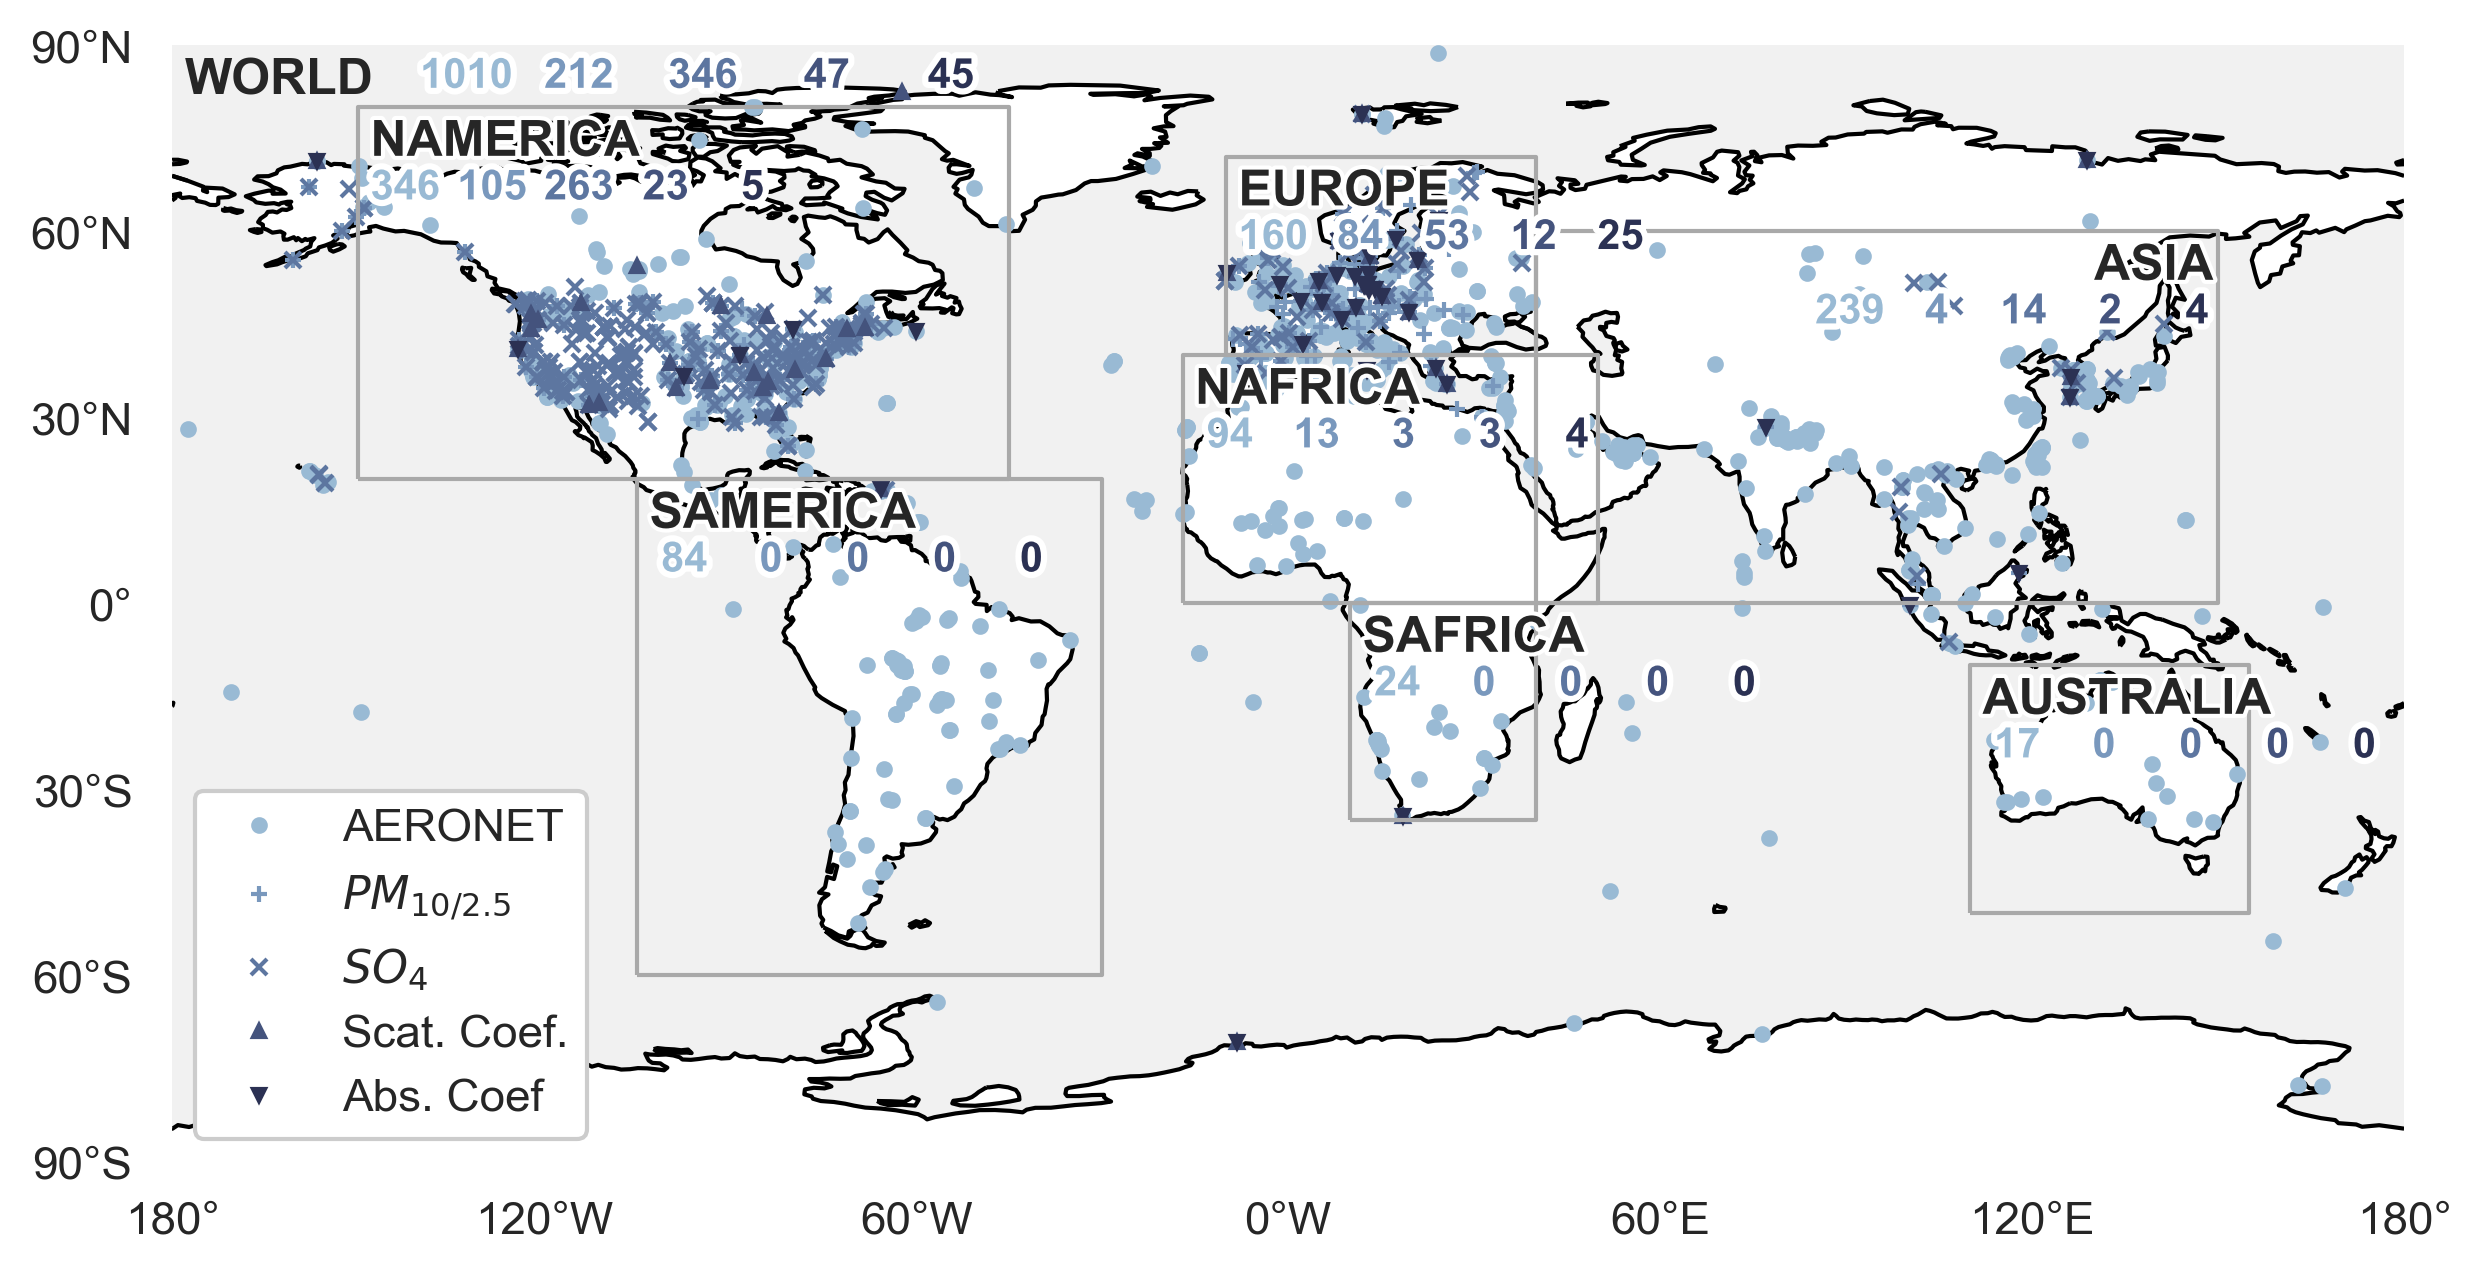
\includegraphics[width=12cm]{../scripts/figs/maps/av_obs.png}
 \caption{Observations and regions used in this study. The numbers reported within each region correspond to the maximum number of stations given for each observation network.}
 \label{fig:map_obs}
\end{figure}

\subsubsection{Constrains}
Common filtering among all the parameters on each station data: use the highest quality level available, remove outliers.

The regional time series are computed by combining, for each timestamp, the valid data of all the station in the corresponding region, for the same timestamp.
In order to compute consistent and robust regional time series, some additional constrains have been applied to the data:
\begin{itemize}
 \item The mountains sites (elevation>1000? m) have been removed.
 \item In order to filter ephemera stations (e.g AERONET DRAGON stations), a minimum of 300 days with valid measurements is required per station, when daily measurements are available.
 \item A minimum of three points (stations with valid measurement) is required per timestamp.
\end{itemize}

When those criteria are fulfilled, the median, the first and third quartiles are computed at the finest time-resolution available. The quartiles allow to capture the inter-regional variability. An example of regional time-series is shown in Figure \ref{fig:ts_aod} for the AOD.

\begin{figure}
 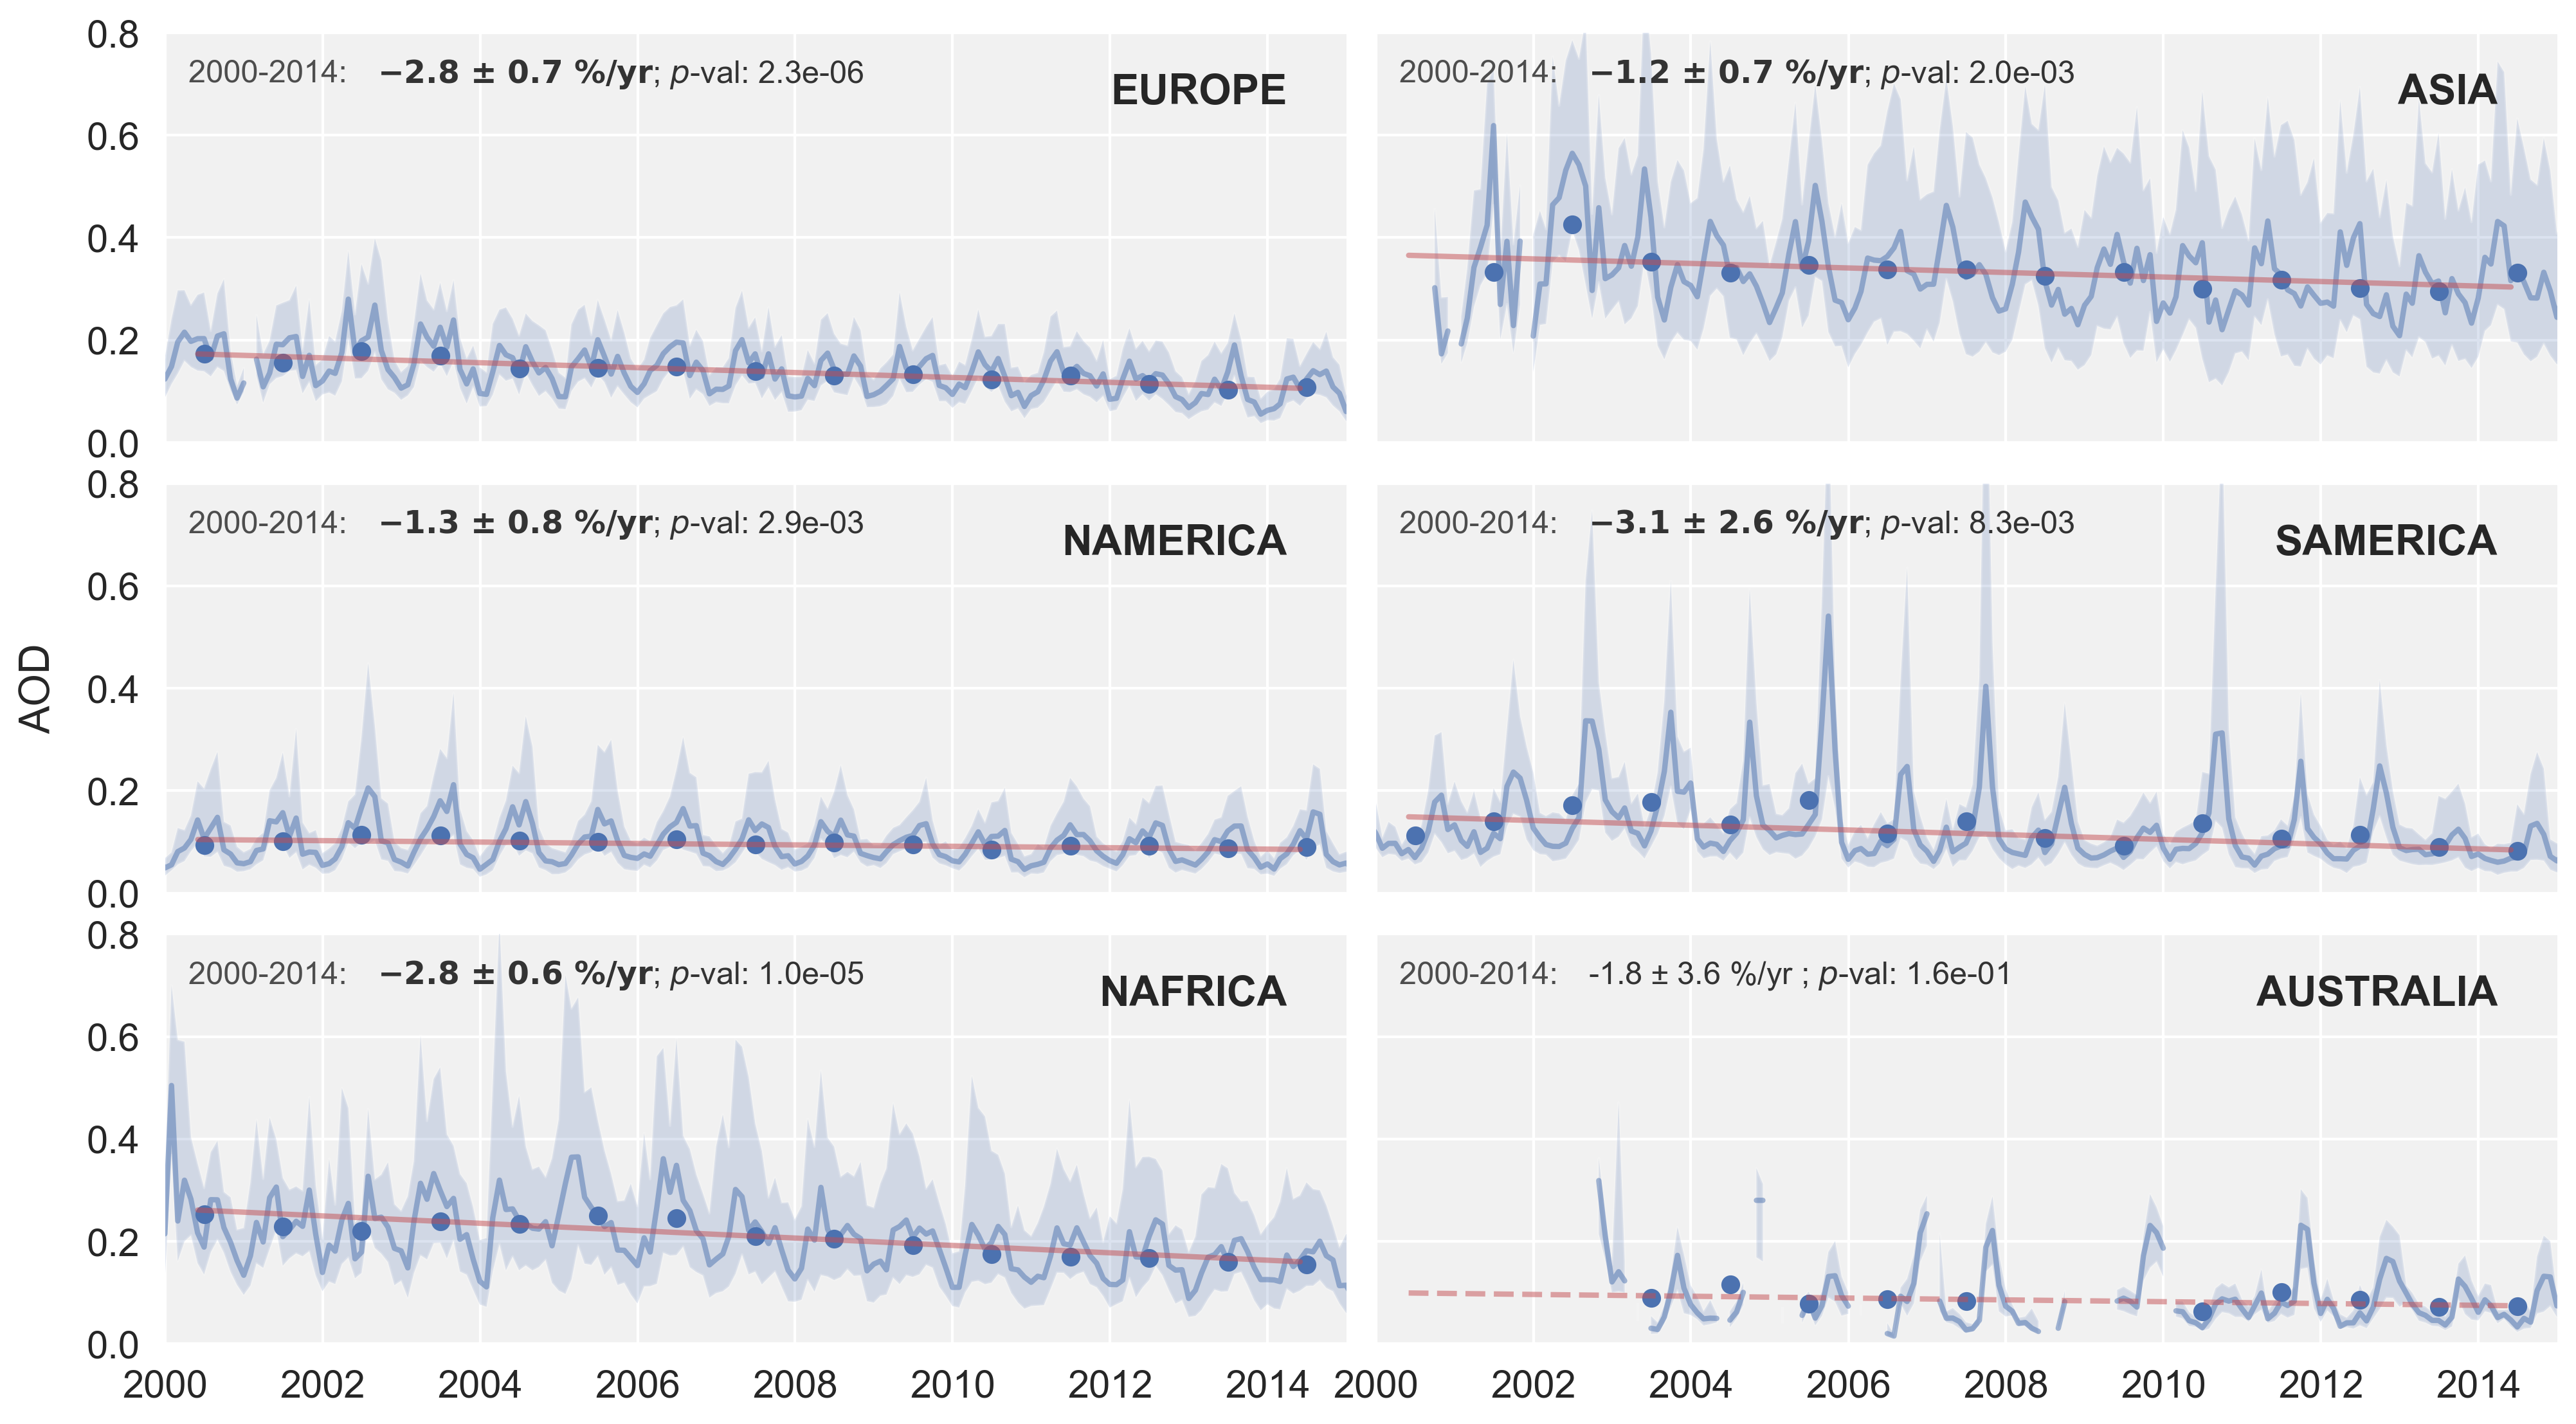
\includegraphics[width=16cm]{../scripts/figs/ts/panel-od550aer.png}
 \caption{Regional time series of AOD. The dark blue line and the light blue envelope correspond respectively to the median and the first and third quartiles of all the valid points at the corresponding timestamp. The blue dots correspond to the yearly averages which are used to compute the linear trend, displayed as a continuous or dashed line when the trend is significant or not.}
 \label{fig:ts_aod}
\end{figure}


\subsection{Trends calculation}

\subsubsection{Regional time series computation}
The trends are processed based on the yearly averages of the regional time series. Using the yearly averages allows to get rid of the seasonal cycles, which are observed in most of the aerosol parameters used in this study, which disturb the calculation of the trend slope. In order to insure the statistical robustness of these yearly average, the time averaging is performed step-by-step with specific time constrains. By starting at the finest time resolution available in the data, monthly, seasonal and yearly averages are computed when the following criteria are fulfilled:
\begin{itemize}
 \item at least 5 days per month (when daily observations are available).
 \item at least 1 month per season.
 \item at least 4 seasons per year.
\end{itemize}
This gives a reasonable compromise between the availability of the measurements and the robustness of the yearly statistics.

\subsubsection{Trends computation}
Same methodology as in \cite{aas2019global}.
Use of yearly averages. Computation if at least 7 points in the time series (50\% of time coverage). That's why, even though 25 stations provide AOD measurements in SAFRICA, no trend is provided in this region since the regional time series contains only 6? points (clean up the website). The trends are computed similarly for both observation and model datasets. However, for the models providing output every 5 years (in addition to 2014), the minimum number of points has been reduced to 4, so the trends can be computed using the years 2000, 2005, 2010 and 2014 *e.g: OsloCTM*.

Trends significance with Mann-Kendall.
Slope calculation with Theil-Sen estimator.
The uncertainty on the trend is calculated by combining the uncertainty on the Theil-Sen slope estimation with the error on the residuals:

\begin{equation}
 Uncertainty = \sqrt{{\left (\frac{\Delta m}{y(2000)}\right )}^{2} + {\left ( \frac{m \cdot \Delta r}{y(2000)^2}\right )}^{2} }
\end{equation}

where $\Delta m$ is the error on the slope as given by the Theil-Sen estimator with an expectancy of 95\%, $y(2000)$ is the value of the regression line at the year 2000, $m$ is the value of the Theil-Sen slope and $\Delta r$ is the averaged error on the residuals.

The trend is provided as a relative trend (\%/yr) as respect to the first year of the time period (2000).

\subsection{Representativity of the trends}
The number of available points used to compute the regional time series is not constant in time. For a given observation station, the number of points available might vary with time due to the nature of the measurements itself. For instance, sun-photometers are performing measurements in the daytime. Due to seasonal daylight and clouds conditions variations, clear seasonal cycles are observed for AOD when considering the number of observations. The density of the different observation networks is also changing in time. The early development of the different observation networks usually went together with an increase of the number of observation stations. *Henceforth, for sustainability reasons, some networks are considering to reduce the number of stations.* These variations in the number of measurements available is rising the question of the time representativity of the measurements for the computation of the trends.

Associated with this time representativity issue comes the space representativity. The trends are provided for regions in which the data density is not homogeneous. Moreover, within a single region, the observation stations might be located in different types of environment. Stations located in more urban, rural environments, or mostly affected by natural particles might have trends differing from the trend associated with the whole region.

It is then legitimate to wonder if the trends computed at the observation stations, with the available data, are representative for the whole period, and the whole region. In order to investigate both these sources of uncertainty, two studies (time and space) have been conducted using model data. For each of these studies, the trends are computed for one reference ($Ref$) and one experiment ($Exp$) dataset, are then compared together.
\begin{itemize}
 \item Time representativity study
       \begin{itemize}
        \item $Ref_{time}$: Collocation in space and time
        \item $Exp_{time}$: Collocation in space using complete time-series
       \end{itemize}
 \item Space representativity study
       \begin{itemize}
        \item $Ref_{space}$: Collocation in space using complete time-series (=$Exp_{t}$)
        \item $Exp_{space}$: All grid-points in region using full time-series
       \end{itemize}
\end{itemize}

The difference between the relative trends are computed for each parameter and over each region. Those differences are then converted into a score (\unit{\%}) by using a normal distribution $f$ described by a mean $\mu=0$ and a standard deviation of $\sigma=0.5$. For a given parameter $p$ and a region $r$, the Representativity $Rep(p,r)$ is calculated as following

\begin{equation}
 Rep_{space,time}(p, r) = {f\left(\left| trend_{Exp_{space,time}(p, r)}-trend_{Ref_{space,time}(p, r)} \right|\right)}
\end{equation}

For a given representativity study, a difference of 0.0\%/yr as compared to its reference dataset leads to a representativity score of 100\%, and a difference of 0.5\%/yr leads to a score of 50\%.
Finally, the total representativity is computed as the mean of the time and the space scores.

An example of representativity calculation is presented in Appendix \ref{sec:representativity}.


\section{Results}

\subsection{Trends in observations}
This sections presents the trends computed with the observations for the different parameters and over the predefined regions.

\begin{table}
 \begin{tabular}{llllllll}
  \tophline
                                & EUROPE & NAMERICA & SAMERICA & NAFRICA & ASIA & AUSTRALIA \\
  \middlehline
  AOD                           & 0.17   & 0.10     & 0.15     & 0.26    & 0.35 & 0.10      \\
  AOD<1µm                       & 0.14   & 0.08     & 0.12     & 0.11    & 0.18 & 0.05      \\
  AOD>1µm                       & 0.03   & 0.02     & 0.03     & 0.10    & 0.11 & 0.03      \\
  AE                            & 1.44   & 1.46     & 1.30     & 0.72    & 1.06 & 0.97      \\
  $PM_{2.5}$ (\unit{µg.m^{-3}}) & 12.7   & 6.0      & -        & -       & -    & -         \\
  $PM_{10}$ (\unit{µg.m^{-3}})  & 16.8   & 11.5     & -        & 19.6    & -    & -         \\
  $SO_{4}$ (\unit{µg.m^{-3}})   & 2.01   & 1.45     & -        & 2.98    & 1.97 & -         \\
  Scat. Coef. (\unit{Mm^{-1}})  & 29.6   & 23.8     & -        & -       & -    & -         \\
  Abs. Coef. (\unit{Mm^{-1}})   & 2.0    & 2.3      & -        & -       & -    & -         \\
  \bottomhline
 \end{tabular}

 \caption{Observations means for the year 2000 (reference year used for computing the relative trends). The value is extracted as the intercept of the linear trend computed in the 2000-2014 period. Note: with the imposed constrains, no trend could be processed in the South-Africa region.}
 \label{table:obs_2000mean}
\end{table}

In order to compare the trends observed for the set of nine aerosol parameters in a consistent manner, one focus on the relative trends, with the reference set to the year 2000, as the first year of the study period. The means for the year 2000, reported in Table \ref{table:obs_2000mean}, reveal a great inter region variability.

The AOD is more than three times higher in Asia (0.35) than in North-America (0.10). Intermediate values are found in Europe, North-America and Australia, while the second highest load is found in North-Africa (0.26). Usually, the AOD is largely dominated by its fine fraction (AOD<1µm), but it is not the case in North-Africa, where the persistent presence of desert dust makes the coarse mode (AOD>1µm) contribution to the total AOD equivalent to the fine mode contribution. This predominance of coarse particles is also noticeable with the AE which is minimum in this region (0.72).

The PM observations are mostly available in Europe and North-America. $PM_{10}$ are also available in North-Africa, but the stations are mostly located in the Northern part of the region which is less affected by the dust sources as compared to the AERONET stations from this region, also located in desert areas. Both $PM{10}$ and $PM_{2.5}$ are larger in Europe than in North-America, with nevertheless different proportions. In Europe, PM2.5 represent 75\% of the PM10, as compared to 52\% in North-America.

$SO_{4}$ means for the year 2000 ranges between 1.45 and 2.98 \unit{µg.m^{-3}} in North-America and Asia, respectively. Similar means are found in Europe and Asia, around 2 \unit{µg.m^{-3}}.

Analogously to the surface $PM_{10}$ measurements, Scat. Coef. is higher in Europe (29.6 \unit{µg.m^{-3}}) than in North-America (23.8 \unit{µg.m^{-3}}). However, a different pattern is found for Abs. Coef. which presents slightly higher values in the latter region.

\begin{figure}[t]
 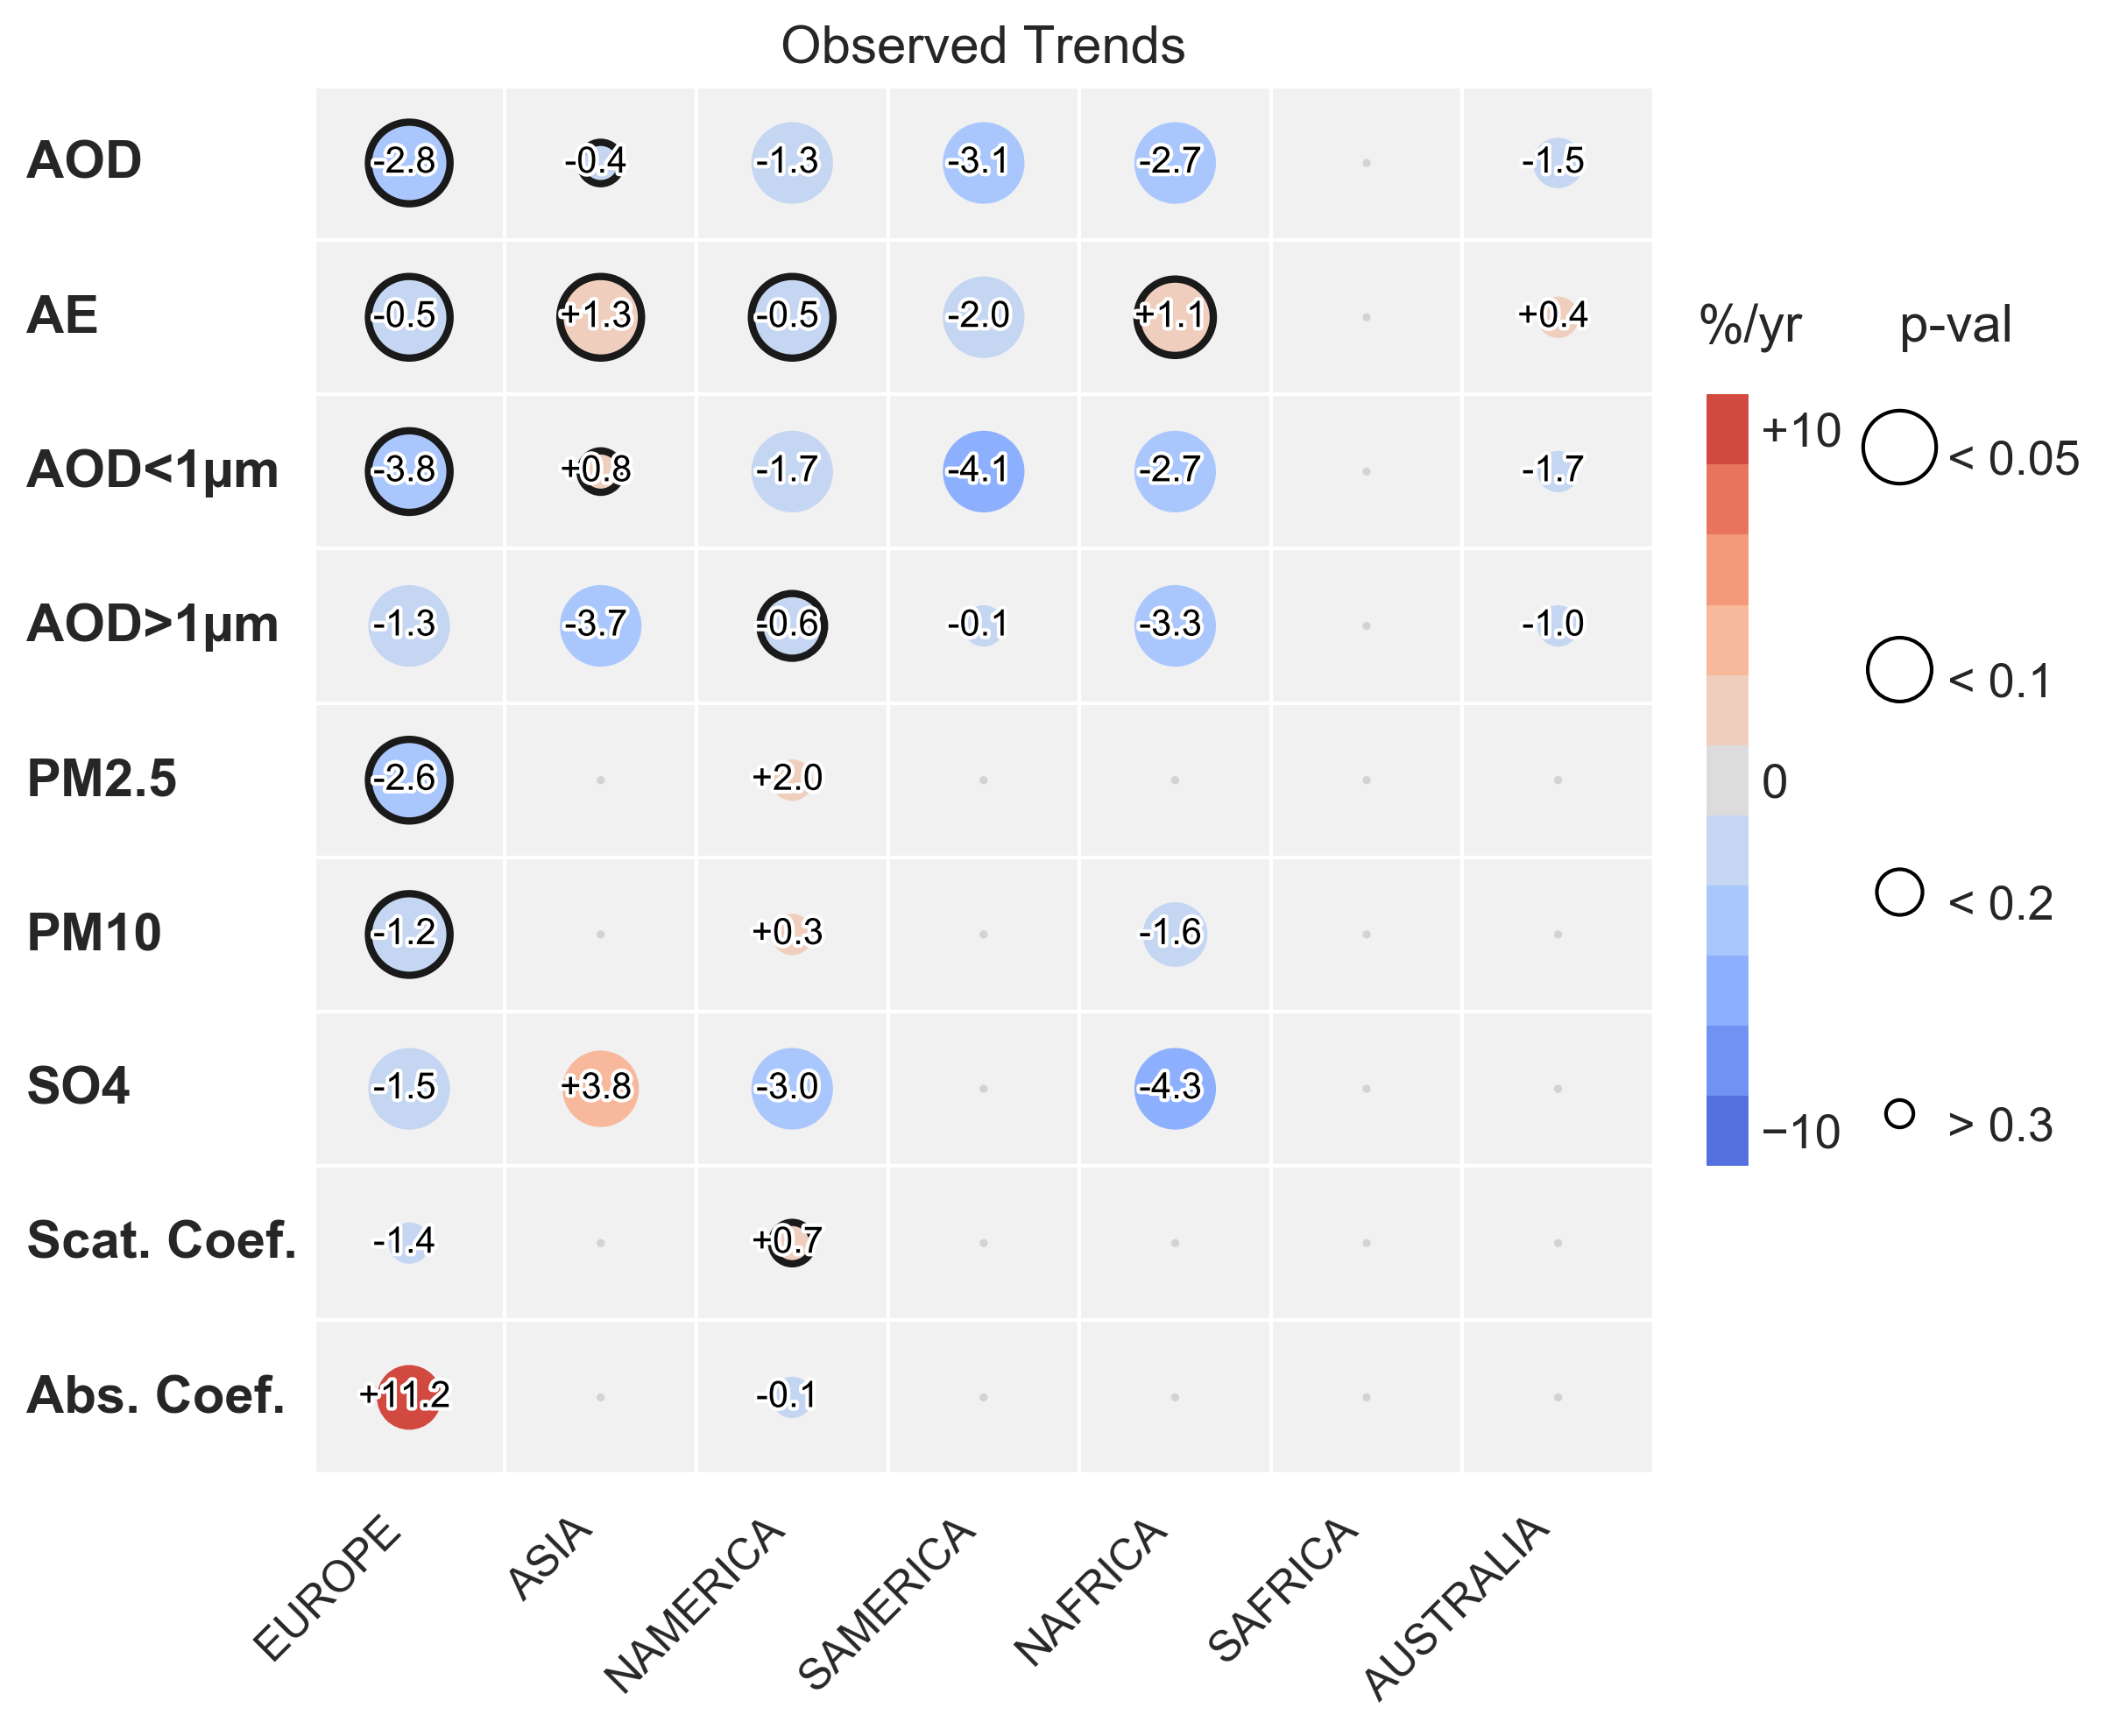
\includegraphics[width=12cm]{../scripts/figs/heatmaps/OBS.png}
 \caption{Regional trends of the aerosol properties computed with the observation datasets. The color of the circles corresponds to the slope, while the radius indicates the p-value. The largest circles represent the trends significant with a confidence of 95\%. The circles bordered with a black line indicate the trends associated with a representativity greater than 50\%.}
 \label{fig:obs_trends}
\end{figure}

The relative trends for the 2000-2014 period are shown in Figure \ref{fig:obs_trends}. The heatmap is dominated by the blue color which indicates mostly negative trends. Usually, the lowest p-values (<0.05) are associated with the lowest uncertainties. The largest circles are then associated with certain decrease/increase since the value of the trend is greater than the uncertainty. Remark: For data coverage reasons, the trends of Scat. Coef. and Abs. Coef., have been computed using data until 2018.

*would need to add some comparisons with published values*
\begin{itemize}
 \item In Europe, both columnar and surface parameters reveal significant decreases, at the exception of Abs. Coef. for which the observed decrease is not significant. For this last parameter, the associated uncertainty on the trend exceed the trend itself. One reason for this large uncertainty is that there is no measurements available prior to 2005. For the other parameters, the uncertainties are lower than the trends. The decrease in AOD (-2.8\%/yr) is found in both fine and coarse modes. The fine mode is decreasing more than the coarse mode, which is consistent with the decrease observed for AE. The same pattern is found at the surface since $PM_{2.5}$ has decrease relatively twice more than $PM_{10}$. These trends could result from mitigation measures aiming for the reduction the anthropogenic aerosols emissions, which is more directly observed with the decrease of $SO_{4}$ (-1.5\%/yr). The representativity study reveals that the observed trends are actually representative for the whole period and region for all of the parameters, at the exception of Scat. Coef. and Abs. Coef. due to the lack of observations in the earliest period.
 \item In North-America, similar trends are found for the columnar properties than in Europe. AOD is decreasing of 1.3\%/yr, so 55\% percent less than in Europe, but the reference value in 2000 is 40\% lower than the reference value in Europe. PM measurements are not available after 2006 within EBAS, which conducts to uncertain trends. $SO_{4}$ decreases about 3\%/yr, which is twice the decrease observed in Europe where the reference value is larger than in North-America. The regional time series are more complete for Scat. Coef. and Abs. Coef. than in Europe. however, no significant trends are found with both datasets. One can note that the observed trends are assessed as representative for the whole period and region for AE, but not for AOD, which have nonetheless the same data availability. This means that the trends are smoother in space and time for AE than for AOD: the type of the particles is changing less than the quantity of these particles.
 \item All of the columnar properties are showing decreasing trends in South-America. All of them being significant, except for AOD>1µm. As shown in the regional time series in \ref{fig:ts_aod}, the decrease observed in AOD comes together with a diminution of the intensity of the seasonal peaks, happening around September. Same patterns are found with AOD<1µm. *Forest Fires? Why does it decrease?*
 \item In North-Africa, while significant decreases are found for all AODs, one observe an increase of AE (+1.1\%/yr), which reveals a greater proportion of fine particles in time. This is consistent when considering the fine and coarse modes, since we observe more important decrease of the coarse particles content.
 \item AE is also increasing in Asia, but seems to result in this case from the combination of a (not significant) increase of AOD<1µm and a significant increase of AOD>1µm. In the meantime, we observe an increase of $SO_{4}$ of 3.8\%/yr. The associated error is however of 4\%/yr. The reason is the presence, in the regional time series, of a few points standing out from the linear regression. These points are associated with a decrease in the number of stations available in the time interval (2010-2012). With a maximum of 12 stations, a few stations missing can affect the computation of the regional time series. This is reflected by the representativity study since the total score is lower than 40\% for this parameter
 \item No significant trends could be found in Australia.

\end{itemize}

\subsection{Evaluation of the models trends against observations}

\begin{figure}[t]
 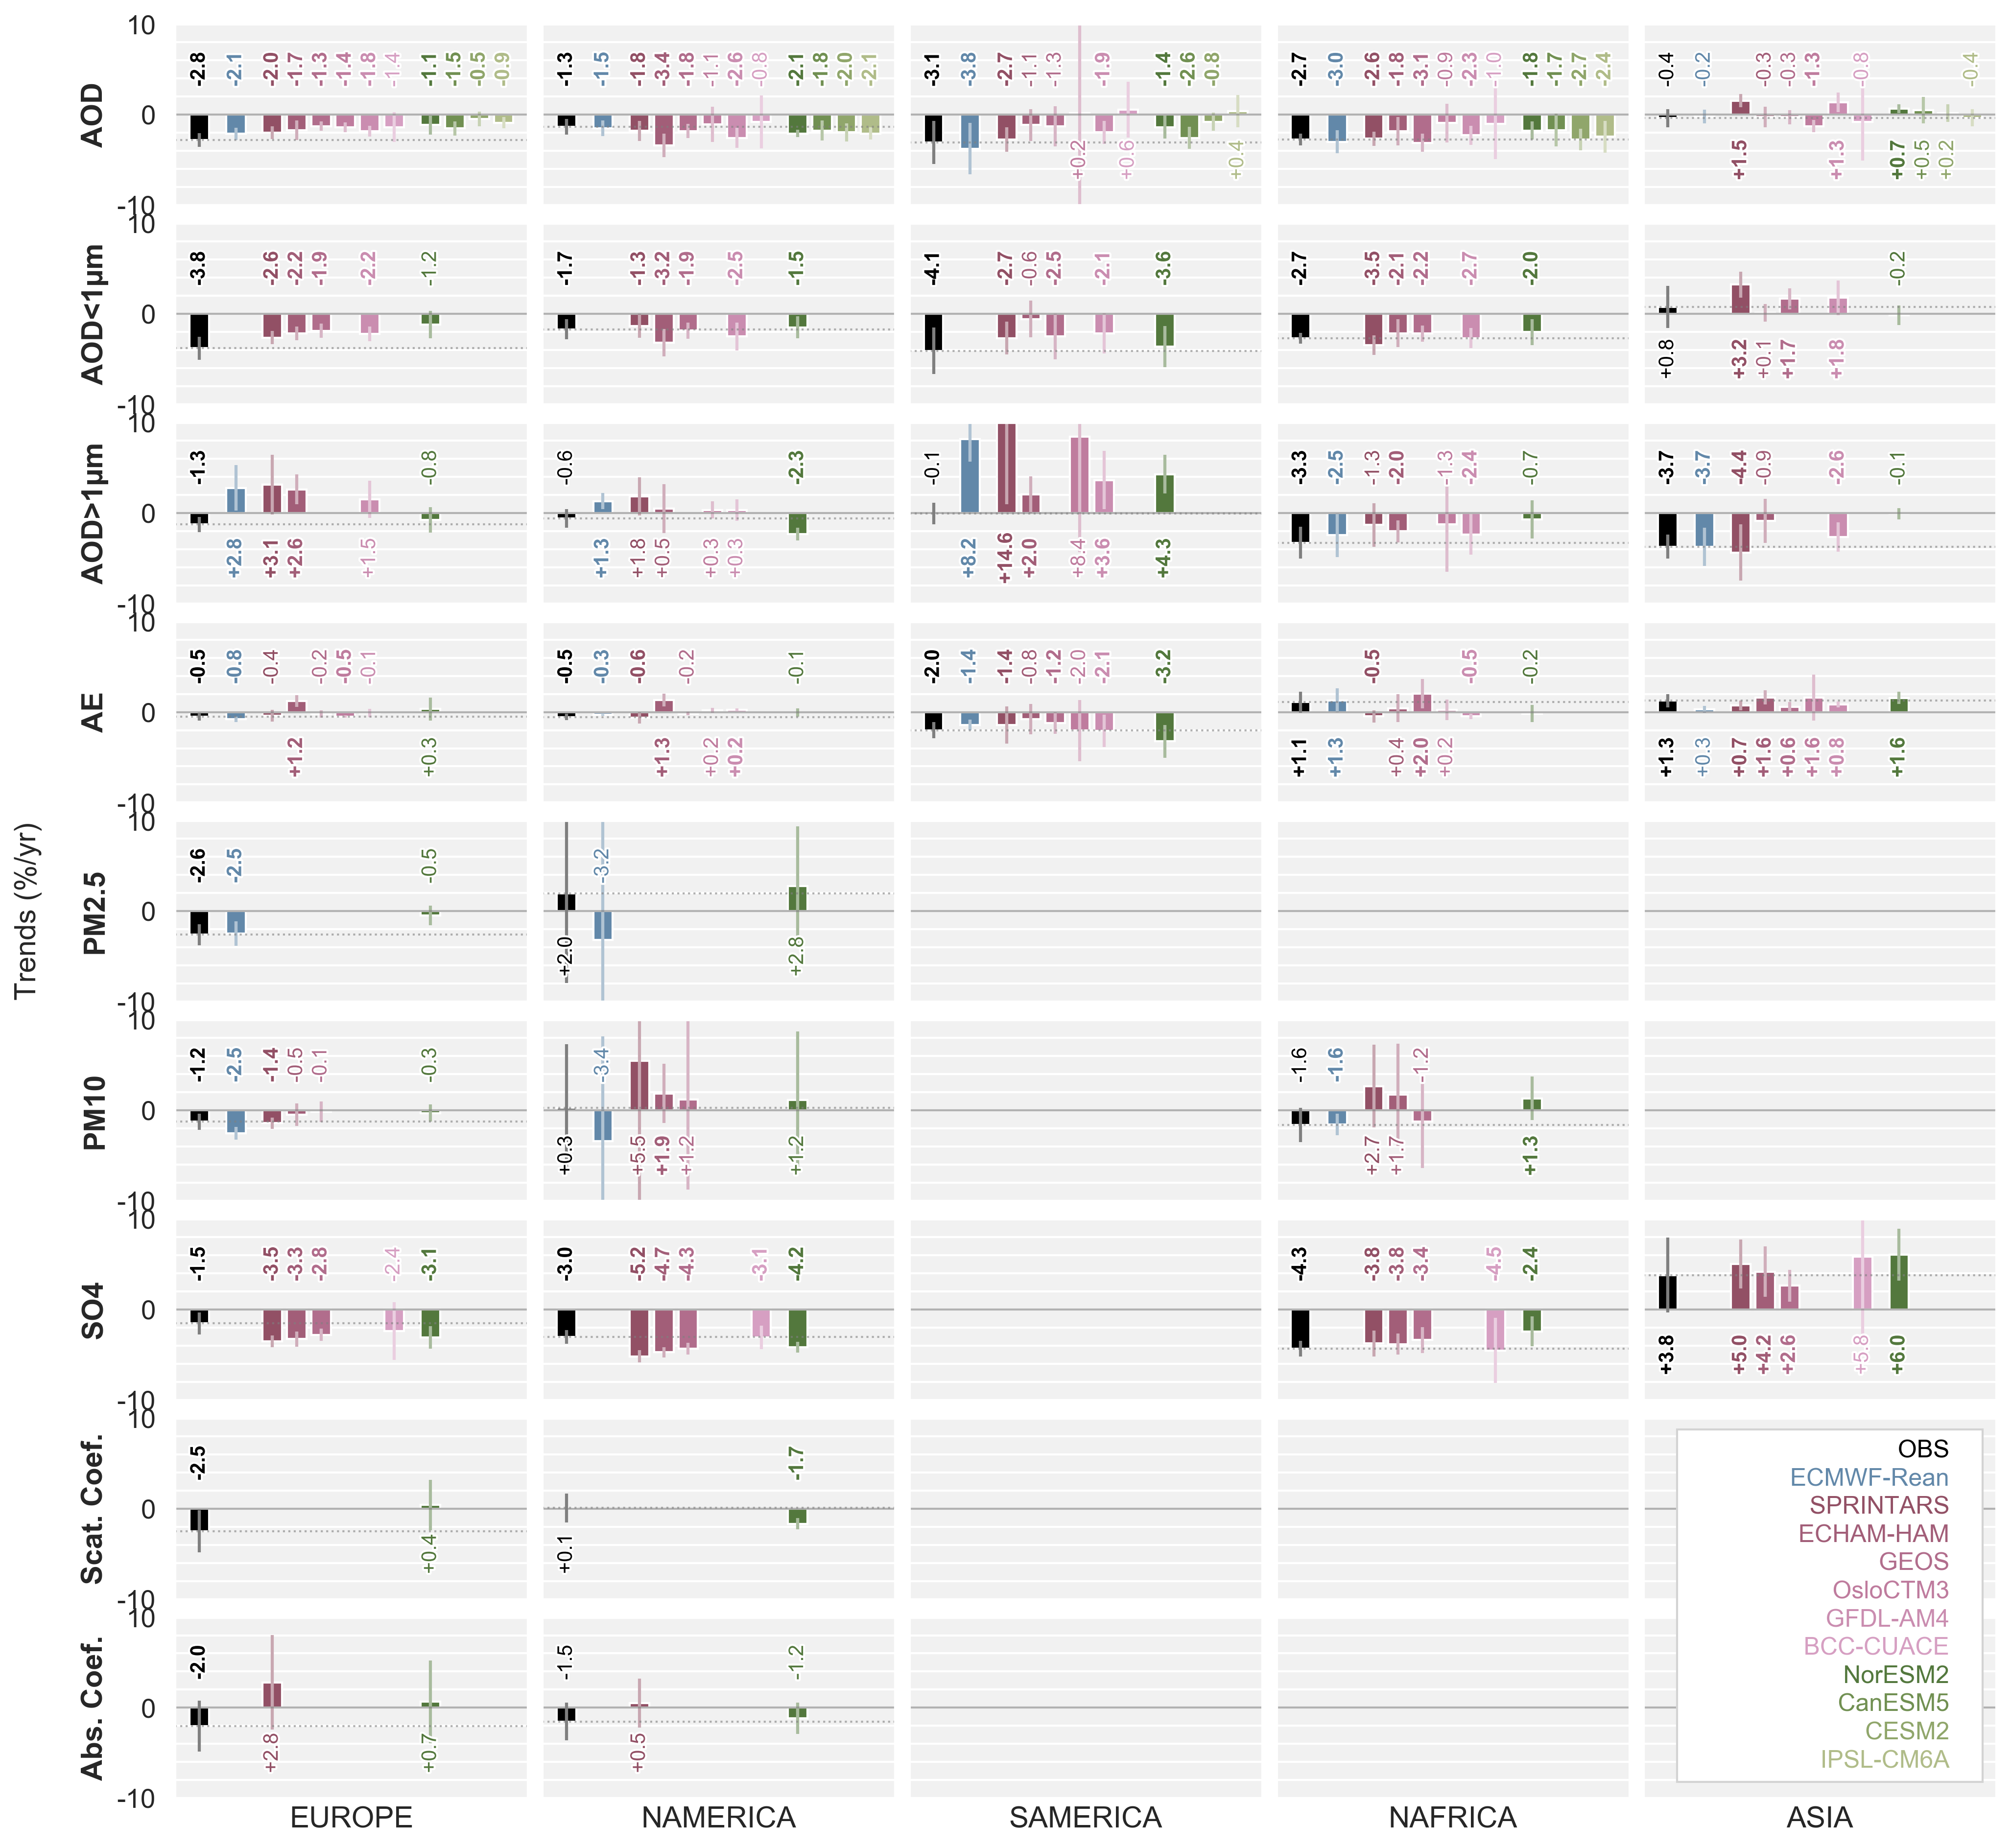
\includegraphics[width=16cm]{../scripts/figs/heatmaps/BARS.png}
 \caption{Regional trends of the aerosol properties computed with observations and models colocated in space and time to the observations. The error bars correspond to the uncertainty of the trend as calculated using both the uncertainty on the Theil−Sen slope and the residuals. The bold font indicates the trends significant with an expectancy of 95\%. *The models are ordered according to the number of output used in this study.*}
 \label{fig:bars}
\end{figure}

In order to evaluate the model trends, the regional time series have been computed with the models output colocated in space and time to the available observations at the stations level. The results are shown in Figure \ref{fig:bars}. The performances of the models, for the reproduction of the observed trends, are various depending on the parameters and the regions.

\begin{itemize}
 \item AOD: the models are showing trends in the same direction than the observation over all the regions except in Asia, where the associated uncertainties are however usually larger than the trends values. Some differences can be noticed in between the three groups of models when investigating the different regions:
       \begin{itemize}
        \item EUROPE: all the groups underestimate the observed decrease. The highest underestimation is observed for the CMIP6 models, with an average decrease of -0.9\%/yr, while the best performance is obtained with CAMS-Rean (-2.0\%/yr). The AP3 models trends are ranging from -0.9\%/yr to -2.1\%/yr.
        \item NAMERICA: at the opposite of EUROPE, on average, all the groups overestimate the observed decrease even though one model of the AP3 group capture lower trends than in the observations. The trends are very close to each other within the CMIP6 group.
        \item SAMERICA: on average, the models perform well in this region. CAMS-Rean, AP3 and CMIP6 show decreases of -3.3\%/yr, -3.1\%/yr and -2.9\%/yr respectively, as compared to -3.1\%/yr for the observations.
        \item NAFRICA: all the models are greatly overestimating the observed decrease trend of -2.7\%/yr. On average, CAMS-Rean and AP3 are giving a decrease of -5.0\%/yr while the CMIP6 models are giving a decrease of -5.9 \%/yr. The regional time series (see website) reveal that most of the models have a large positive ibas prior to 2006, which is dramatically reduced after this year. This change in bias induces a large negative trend in most of the models.
        \item ASIA: All the model groups are showing increasing trends, ranging from +0.3\%/yr to 1.7\%/yr, most of them being significant, which is not visible in the observations due to the large uncertainties.
       \end{itemize}
 \item AOD<1µm: the trends are only available with models from the AP3 group for this parameter. Usually, the same patterns are found than with AOD. The models that were underestimating the AOD are underestimating AOD<1µm and vice versa.
       \begin{itemize}
        \item in EUROPE: the underestimation of the models happens in a larger extent than with AOD.
        \item SAMERICA: the inter model variability within AP3 is lower than for AOD and all of the models are well reproducing the observed trends.
        \item NAFRICA: at the opposite of AOD, one observe an averaged underestimation of the observed trend. The inter model variability is quite high over this region since the trends are ranging from -0.6\%/yr to -2.9\%/yr.
        \item ASIA: an increase, associated to large uncertainties is found in both models and observations.
       \end{itemize}
 \item AOD>1µm: the performances of the models are not as good as for AOD<1µm. The inter model variability is also higher since some models are capturing trends in opposite directions.
       \begin{itemize}
        \item EUROPE: while the observations are showing a significant decrease, CAMS-Rean and three of the AP3 models are showing increasing AOD>1µm.
        \item SAMERICA: CAMS-Rean gives the highest positive significant trend. The regional time series shows that there is a large negative bias in 2003 (the first year available for this model) that has been reduced year after year since. This bias reduction leads to an important increasing trend.
        \item NAFRICA: CAMS-Rean capture well the observed trend. No significant trends are found with AP3 models, which is also visible through the large uncertainties.
        \item ASIA: all the models capture a decrease, however underestimated as compared to the significant decrease given by the observations.
       \end{itemize}
 \item AE: the trends are usually relatively lower than for AOD. This feature is also usually visible in the models.
       \begin{itemize}
        \item EUROPE and NAMERICA: one model of the AP3 group (ECHAM-HAM) is giving significant positive trends while negative values are obtained with other datasets.
        \item SAMERICA: all of the models are giving negative trends, consistently with the observations.
        \item NAFRICA: GEOS is showing a large and significant increase (+16.5\%/yr). The analysis of the time series reveals an important negative bias before the year 2006 (-50\%) while the yearly averages tends to be very close to the observations after this year.
        \item ASIA: significant positive trends are well captured by most of the AP3 models.
       \end{itemize}
 \item PM2.5: because PM observation are available after 2006 in North-America, the trends are associated with large uncertainties which makes the validation difficult in this region. However, regardless these uncertainties, the trends seem to be well captured by NorESM2, from the AP3 group, in this region. In Europe, CAMS-Rean is well capturing the trends in the observations.
 \item PM10: CMAS-Rean is reproducing well the observed decrease in North-Africa, but overestimates the decrease in Europe. The variability is quite high with the AP3 group. In North-Africa, most of the models are showing an increase, at the opposite direction of the observed trends.
 \item $SO_{4}$: *look at some values from \cite{aas2019global}*. The AP3 models perform pretty well for the SO4 surface concentration. The extent of the trends are however higher than the observed ones in all the regions at the exception of North-Africa.
 \item Scat. Coef. and Abs. Coef.: as mentioned in the previous section, the observations trends have been computed for these two parameters using data until 2018. The two models providing output for these parameters are NorESM and SPRINTARS. The first model provides data until 2014, so the trends have been computed for [2000-2014], while the second one provides data until 2018 and then covers the whole observation period [2000-2018]. The trends might differ in between these two periods.
       \begin{itemize}
        \item EUROPE: a significant decrease is found in Scat. Coef. observations, which is not captured by NorESM2. For Abs. Coef., the uncertainties are larger than the trends values. Nevertheless, observations and models are capturing opposite trends.
        \item NAMERICA: A significant decrease is found with NorESM2 for Scat. Coef. which is not visible in the observations. For Abs. Coef, the two models are capturing opposite and uncertain trends.
       \end{itemize}
\end{itemize}

*What is happening in Africa in the models before 2006?*

\subsection{Trends in models}

\subsubsection{Global trends}

\begin{table}
 \begin{tabular}{lll}
  \tophline
                                & $Mean_{2000}$ & Trend (\%/yr) \\
  \middlehline
  AOD                           & (0.16) 0.14   & (+0.1) +0.2   \\
  AOD<1µm                       & (0.09) 0.05   & (+0.4) +0.6   \\
  AOD>1µm                       & (0.06) 0.09   & (-0.2) +0.1   \\
  AE                            & (0.78) 0.43   & (+0.2) +0.3   \\
  $PM_{2.5}$ (\unit{µg.m^{-3}}) & (12.4) 9.1    & (+0.2) +0.2   \\
  $PM_{10}$ (\unit{µg.m^{-3}})  & (19.3) 18.7   & (+0.1) +0.1   \\
  $SO_{4}$ (\unit{µg.m^{-3}})   & (2.33) 0.64   & (-1.1) +0.4   \\
  Scat. Coef. (\unit{Mm^{-1}})  & (28.0) 21.2   & (+0.3) +0.2   \\
  Abs. Coef. (\unit{Mm^{-1}})   & (3.1) 0.9     & (+1.8) +1.5   \\
  \bottomhline
 \end{tabular}
 \caption{Global means and trends of aerosol parameters using NorESM2 data. The value in parenthesis is obtained by aggregating only grid-points where observation stations are located while using the complete model time series. The relative trends are calculated by averaging the absolute trends within the considered grid-points and normalizing it to the global mean for the year 2000.}
 \label{table:global_trends}
\end{table}

\begin{figure}[t]
 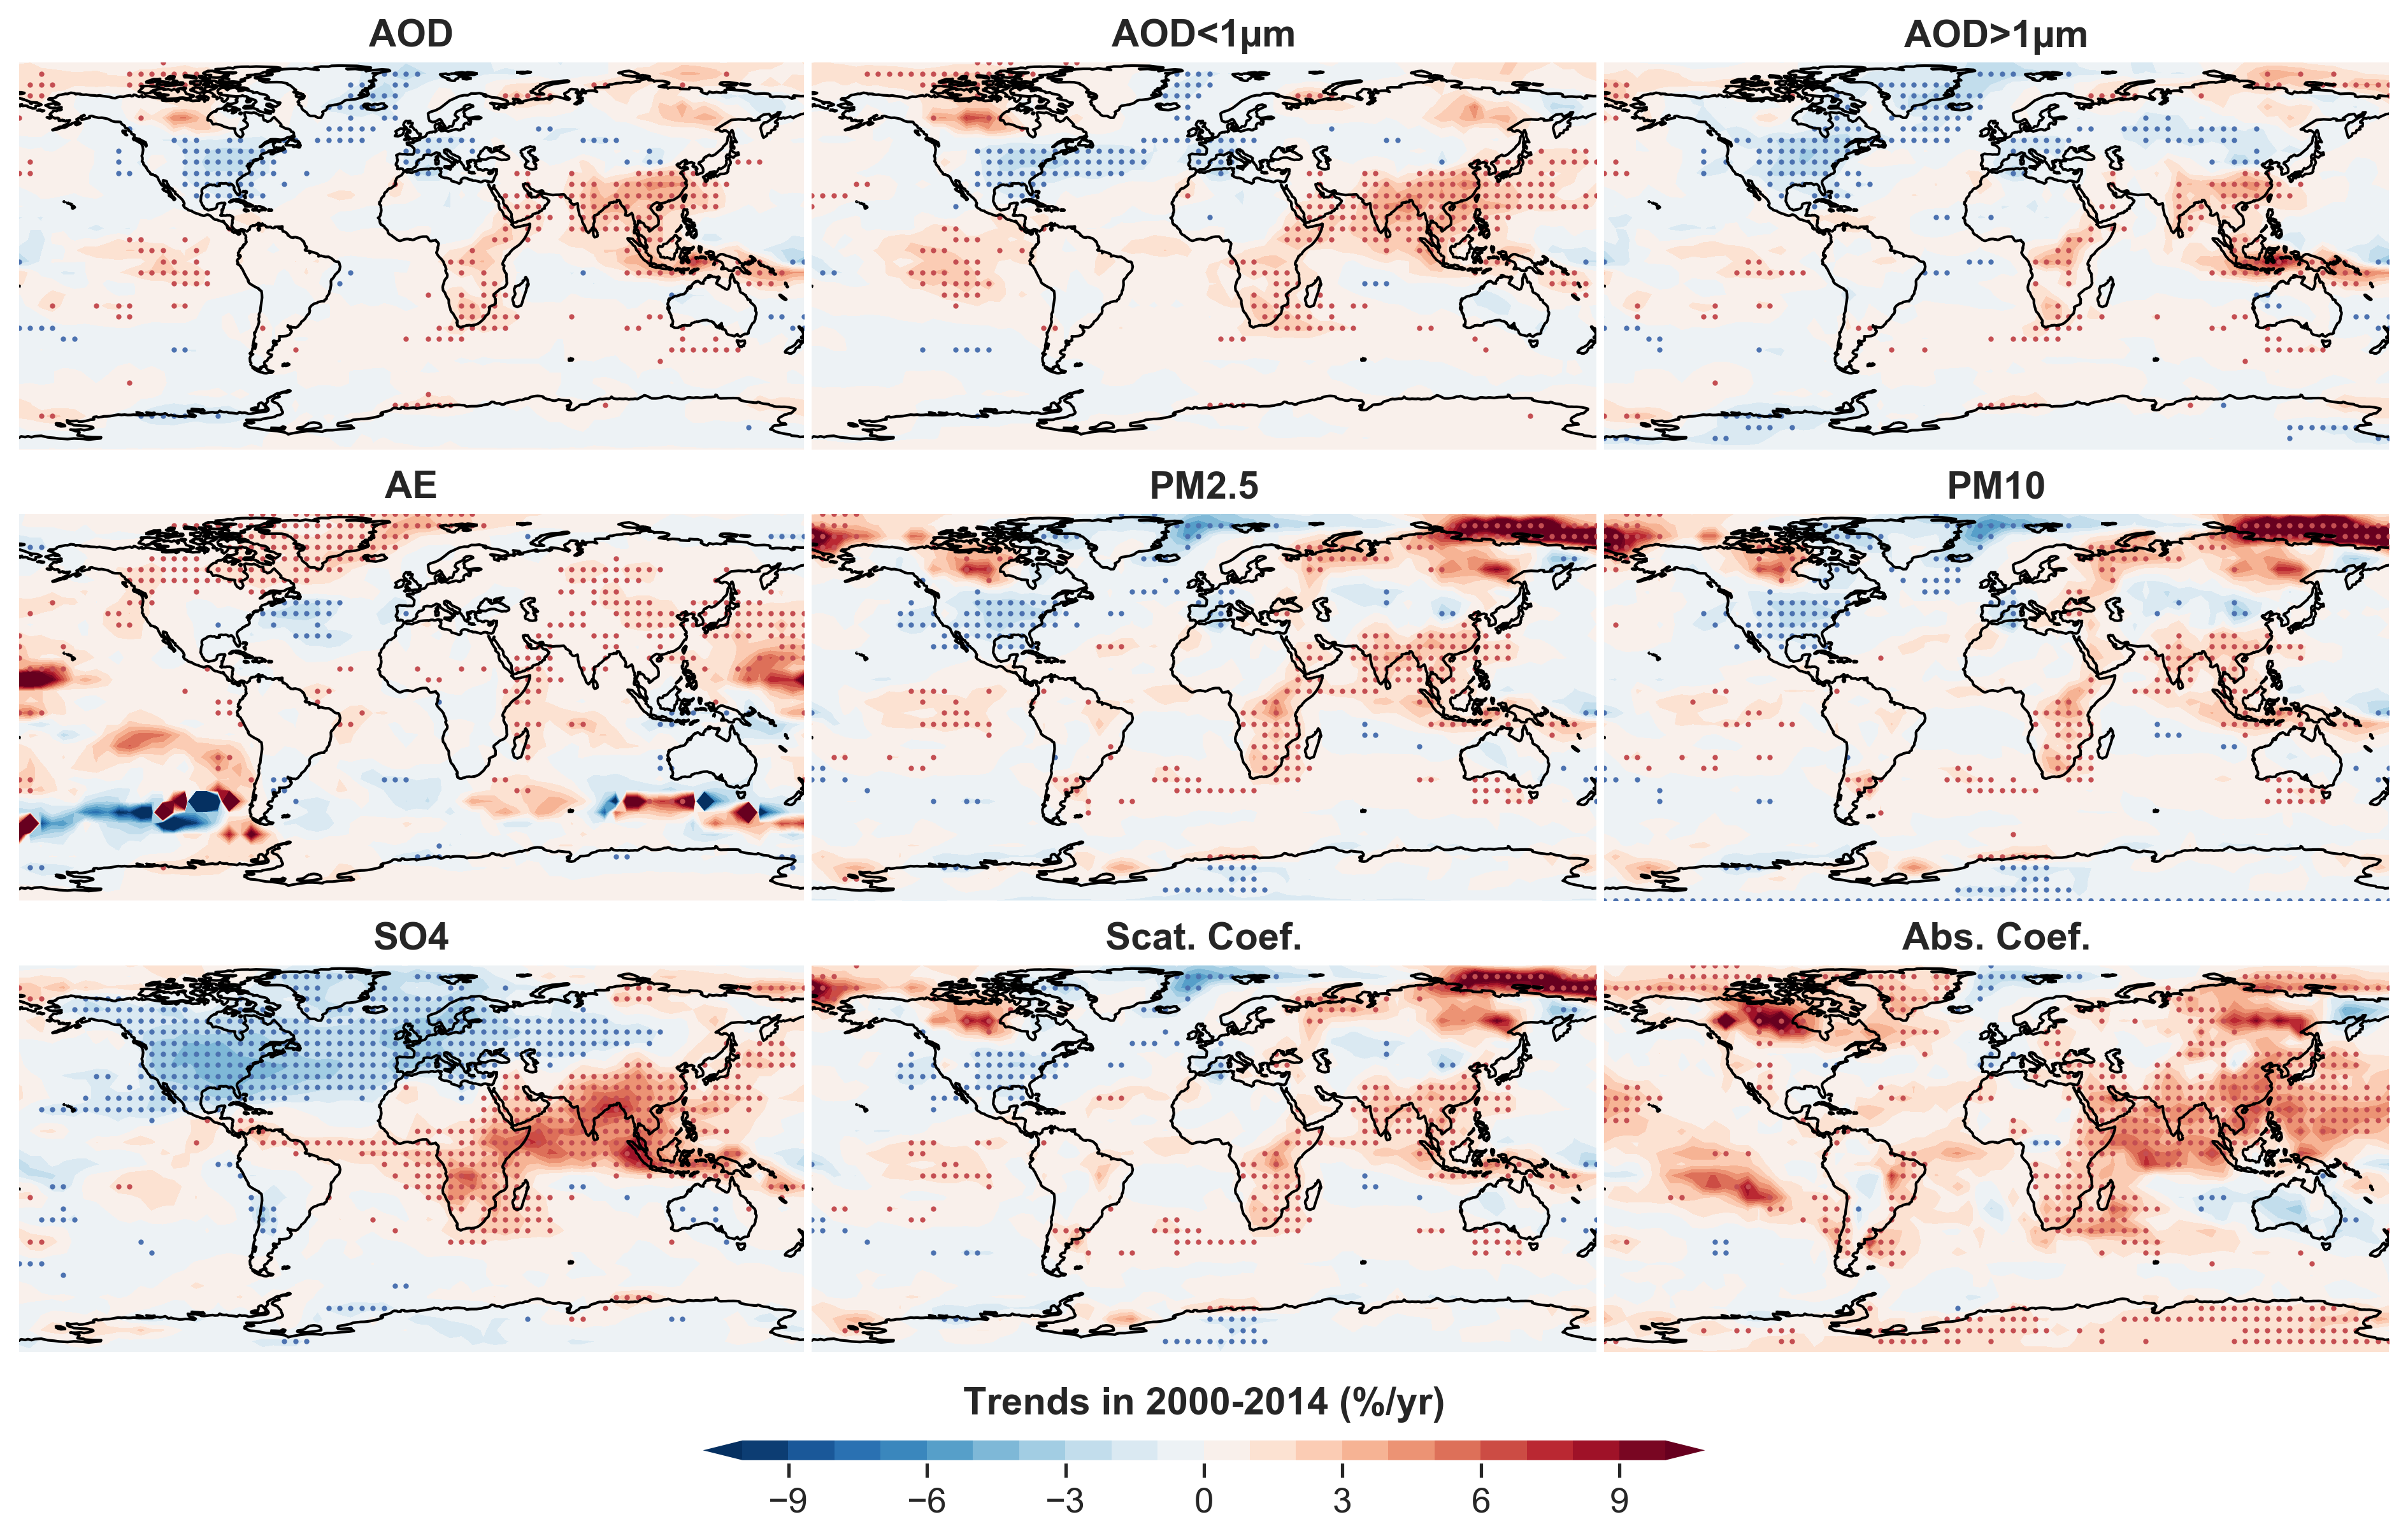
\includegraphics[width=16cm]{../scripts/figs/trends_map2.png}
 \caption{Global trends of aerosol properties using NorESM2 data regridded at a 5x5 degrees resolution. The blue and red dots dots indicate respectively significant negative and positive trends, regardless the colorscale.}
 \label{fig:global_trends}
\end{figure}

As shown in Figure \ref{fig:obs_trends}, the regional trends presented previously are not always representative of the actual trends happening in the entire regions and over the whole study period. The reasons are the partial spacial and time coverage of the ground based observations. Moreover, the observation stations are obviously located over land, which does not permit to depict a global picture of the aerosol trends, while the sea salts represent one of the largest fraction (*reference*) of the aerosols on Earth.

In order to provide a more complete picture of the aerosols at a global scale, we present, in this section, the trends computed with the NorESM2 data (AP3 group) at a global scale. The calculation of the global trends is made by averaging the absolute trends at each grid-point of the model, and scaling it down to the global average for the year 2000. The global trends are reported for the nine aerosol parameters in Table \ref{table:global_trends}. The global maps, shown in Figure \ref{fig:global_trends}, allow to investigate the spatial variability of these trends.

While the observed trends in the three AODs are showing a decrease in most of the regions of the World, the global AOD trend is actually positive (+0.2\%/yr). The increase is the most important for the fine fraction, with and increase of about +0.6\%/yr as compared to +0.1\%/yr for AOD>1µm. As seen in Figure \ref{fig:global_trends}, similar patterns are found for the three AODs: increase in South-Africa and East-Asia. and decrease in Europe and in the US. The increasing AOD observed in Canada is dominated by an increase of AOD<1µm in this region. The important increase observed for AOD in Indonesia seem to be linked with a large increase of AOD>1µm. In the Pacific, an area is presenting significant positive trends, in both AOD and AOD<1µm. Almost no significant trend is found below 60\textdegree S of latitude.

AE is also increasing  at a global scale, with a rate of +0.3\%/yr. The increases happen mostly over the Canada, Greenland, in Syberia and over the Pacific ocean. One observe some outliers around the latitude of 60\textdegree S.
IN the Atlantic, one observe a decrease of AE, which can be linked to the decrease observed for AOD<1µm in the same area.

Both $PM_{2.5}$ and $PM_{10}$ present similar geographical patterns than AOD. In addition, one observe a large and significant increasing trend area in the North Pole. The global averages show that $PM_{2.5}$ is increasing faster than $PM_{10}$  (+0.2\%/yr VS +0.1\%/yr), which is consistent with the increasing AE.

The surface $SO_{4}$ concentration shows two large contrasted regions. Significant decrease are found in North-America and Europe, while significant increases are found in South-Africa and Asia. This contrast illustrates the transfer of the polluting activities from developed countries to the countries in development operated over the last two decades. With an increase of +0.4\%/yr, the global trend is positive.

The Scat. Coef. trends are almost identical to the PM maps. The global trend is also similar since the increase is assessed as +0.2 \%/yr for the studying period.

Abs. Coef. reveals increasing trends over most of the grid-points of the model. This explains the largest global obtained for this parameter, with a global increase of +1.5\%/yr.

The Table \ref{table:global_trends} contains also the trends computed for the different aerosol parameters when combining only the grid-points where an observation station is located. The difference with the trends presented in the previous section is that the complete time series are used in this case, which might conduct to major differences for the resulting datasets, then leading to significantly different trends. This is particularly the case for $SO_{4}$ for which the observation stations are located mostly in Europe and North America, in the large decreasing area while only few stations are located in the regions associated with increasing values. This conducts to a global decrease of -1.1\%/yr when focusing only at the points where observations stations are located, while an increasing trend of +0.4\%/yr is actually obtained when considering all of the grid-points.


\subsubsection{Can we explain the trends in AOD?}

\begin{figure}[t]
 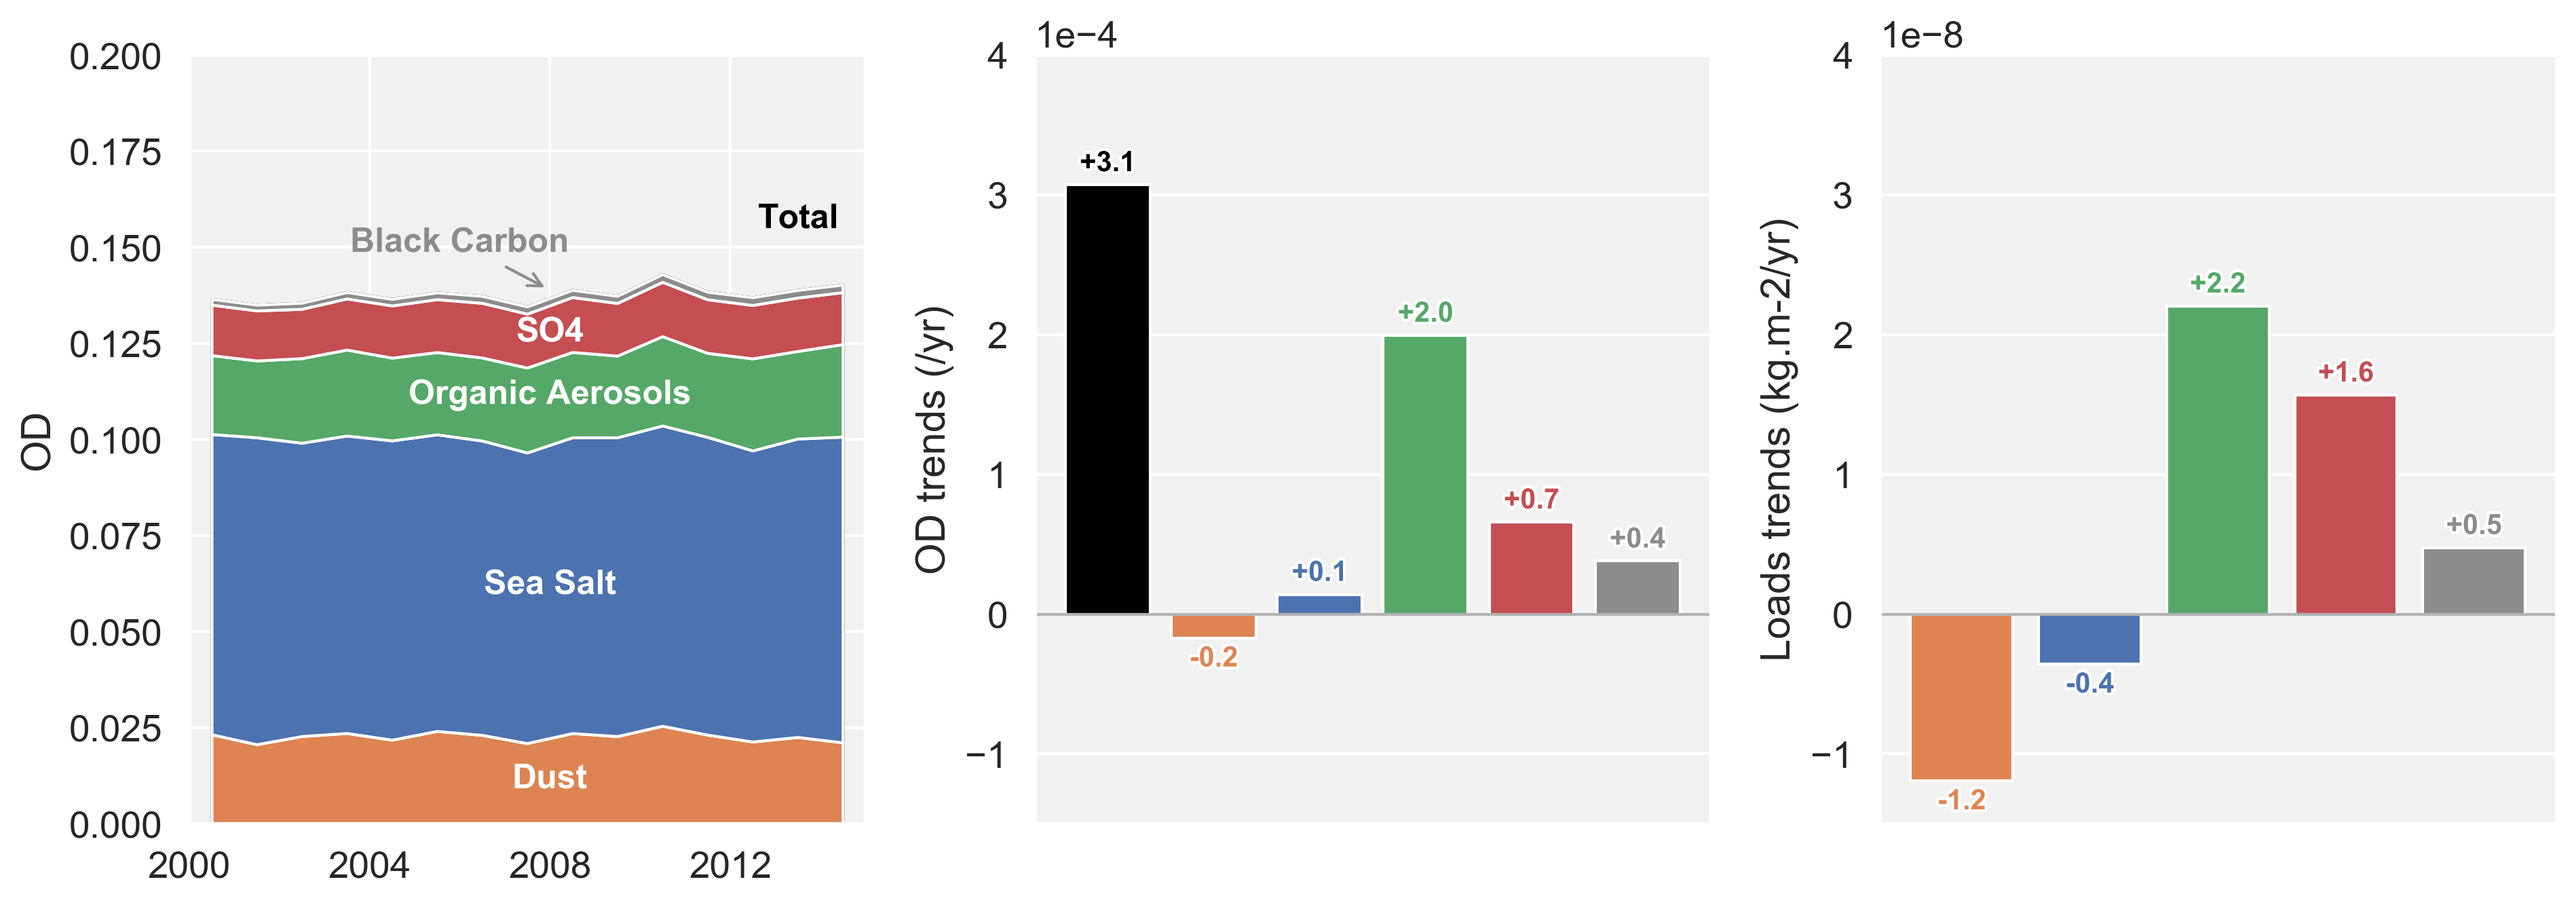
\includegraphics[width=16cm]{../scripts/figs/abs_species_trends.png}
 \caption{Absolute trends in OD and emissions of the main aerosol species computed with NorESM2. The y-axis of the trends in OD and the emissions is given according to the power of 10 indicated at the top left corner of each of these subplots.}
 \label{fig:species}
\end{figure}

The global trends indicate that AOD is increasing in the 2000-2014 period with a rate of about 0.2\%/yr. The trends in AE, AOD<1µm and AOD>1µm indicate that the fine particles are mostly responsible of this trend in the atmospheric column.

In this section, on investigates the trends of the different major aerosol species simulated by the models. In that purpose, the absolute trends have been compute for the contribution of these species to the AOD, as well as for their emissions. The results are shown in Figure \ref{fig:species}.

The relative increase of +0.2\%/yr corresponds to an absolute increase of +3.1e-4/yr. This positive trend is dominated by the trends in Organic Aerosols (OA), SO4 and Black Carbon, which are responsible for increases of the OD of about +2.0e-4/yr, +0.7e-4/yr and +0.4e-4/yr. On average, the contribution of the dusts and sea salts is slightly negative (-0.1e-4/yr).

Link with emissions

\begin{table}[]
 \centering
\begin{tabular}{llll}
\tophline
Species & OD (\%/yr) & Emissions (\%/yr) & Load (\%/yr) \\
\middlehline
   dust &      -0.13 &             -0.55 &        -0.18 \\
     ss &      +0.02 &             +0.01 &        -0.02 \\
     oa &      +1.09 &             +0.52 &        +0.67 \\
    so4 &      +0.61 &             -0.17 &        +0.91 \\
     bc &      +2.28 &             +1.89 &        +2.21 \\
\bottomhline
\end{tabular}
 \caption{Relative trends of the major aerosol species computed with NorESM2.}
 \label{tab:species}
\end{table}




\conclusions  %% \conclusions[modified heading if necessary]
In summary:
- observed trends: mostly decreasing. Some networks give representative trends for the whole region and for the whole period. Some others don't.
- the models manage to reproduce the observed trends..
- global trends using model data give a different picture than when using ground-based observations. Because only land stations, and also not the same coverage in between the different regions.
- global trends show mostly increase, dominated by a larger increase of the fine particles, in the column and also at the surface. This increase seem to be dominated by the organic aerosols, whose emission has increased in the study period. Also, SO4 OD is increasing as well as its load, even though the emissions did not change significantly.

Some perspective:
\begin{itemize}
 \item Ground based observation networks are more or less representative for computing regional trends.
 \item The models reproduce pretty well the observed trends. Some examples with best/worst match.
 \item Great differences in global trends when considering only observation stations or using all grid-points --> Use of satellites. How long are the time series now?
 \item What about seasonal trends? For instance, AOD time series for SAMERICA reveal strong cycles for which the local maximum is decreasing significantly in time. The trend could be driven by a decrease of the extreme events *Is it consistent with the expected increasing forest fires?*
 \item also, trends in meteorological parameters (wind speed, humidity)?
\end{itemize}


%% The following commands are for the statements about the availability of data sets and/or software code corresponding to the manuscript.
%% It is strongly recommended to make use of these sections in case data sets and/or software code have been part of your research the article is based on.

\codeavailability{TEXT} %% use this section when having only software code available


\dataavailability{TEXT} %% use this section when having only data sets available


\codedataavailability{TEXT} %% use this section when having data sets and software code available


\sampleavailability{TEXT} %% use this section when having geoscientific samples available


\videosupplement{TEXT} %% use this section when having video supplements available


\appendix
\section{Representativity study} \label{sec:representativity} %% Appendix A

The Figure \ref{fig:representativity} shows an example of the repesentativity of the AOD measurements in Europe and North-America for the computation of the trends in 2000-2014.

In both regions, the $Ref_{t}$ dataset reveals strong seasonal cycles for the number of points used to compute the regional time-series. This comes from the nature of the AOD measurements, which are obtained during daytime, while amount of daylight is minimum in wintertime in the Northern Hemisphere. Together with this seasonal cycle, one observe an increase in time of the number of points, which reflect the increasing number of stations within each region.

The ocean grid-points are not filtered out while computing the representativity of the different parameters in the different regions of the World. For this reason, the regions containing a greater proportion of ocean grid-points, where the trends are most likely to differ from the trends observed over land, will tend to have a lower spatial representativity.

\subsection{}     %% Appendix A1, A2, etc.


\noappendix       %% use this to mark the end of the appendix section

%% Regarding figures and tables in appendices, the following two options are possible depending on your general handling of figures and tables in the manuscript environment:

%% Option 1: If you sorted all figures and tables into the sections of the text, please also sort the appendix figures and appendix tables into the respective appendix sections.
%% They will be correctly named automatically.

%% Option 2: If you put all figures after the reference list, please insert appendix tables and figures after the normal tables and figures.
%% To rename them correctly to A1, A2, etc., please add the following commands in front of them:


\begin{figure}[t]
 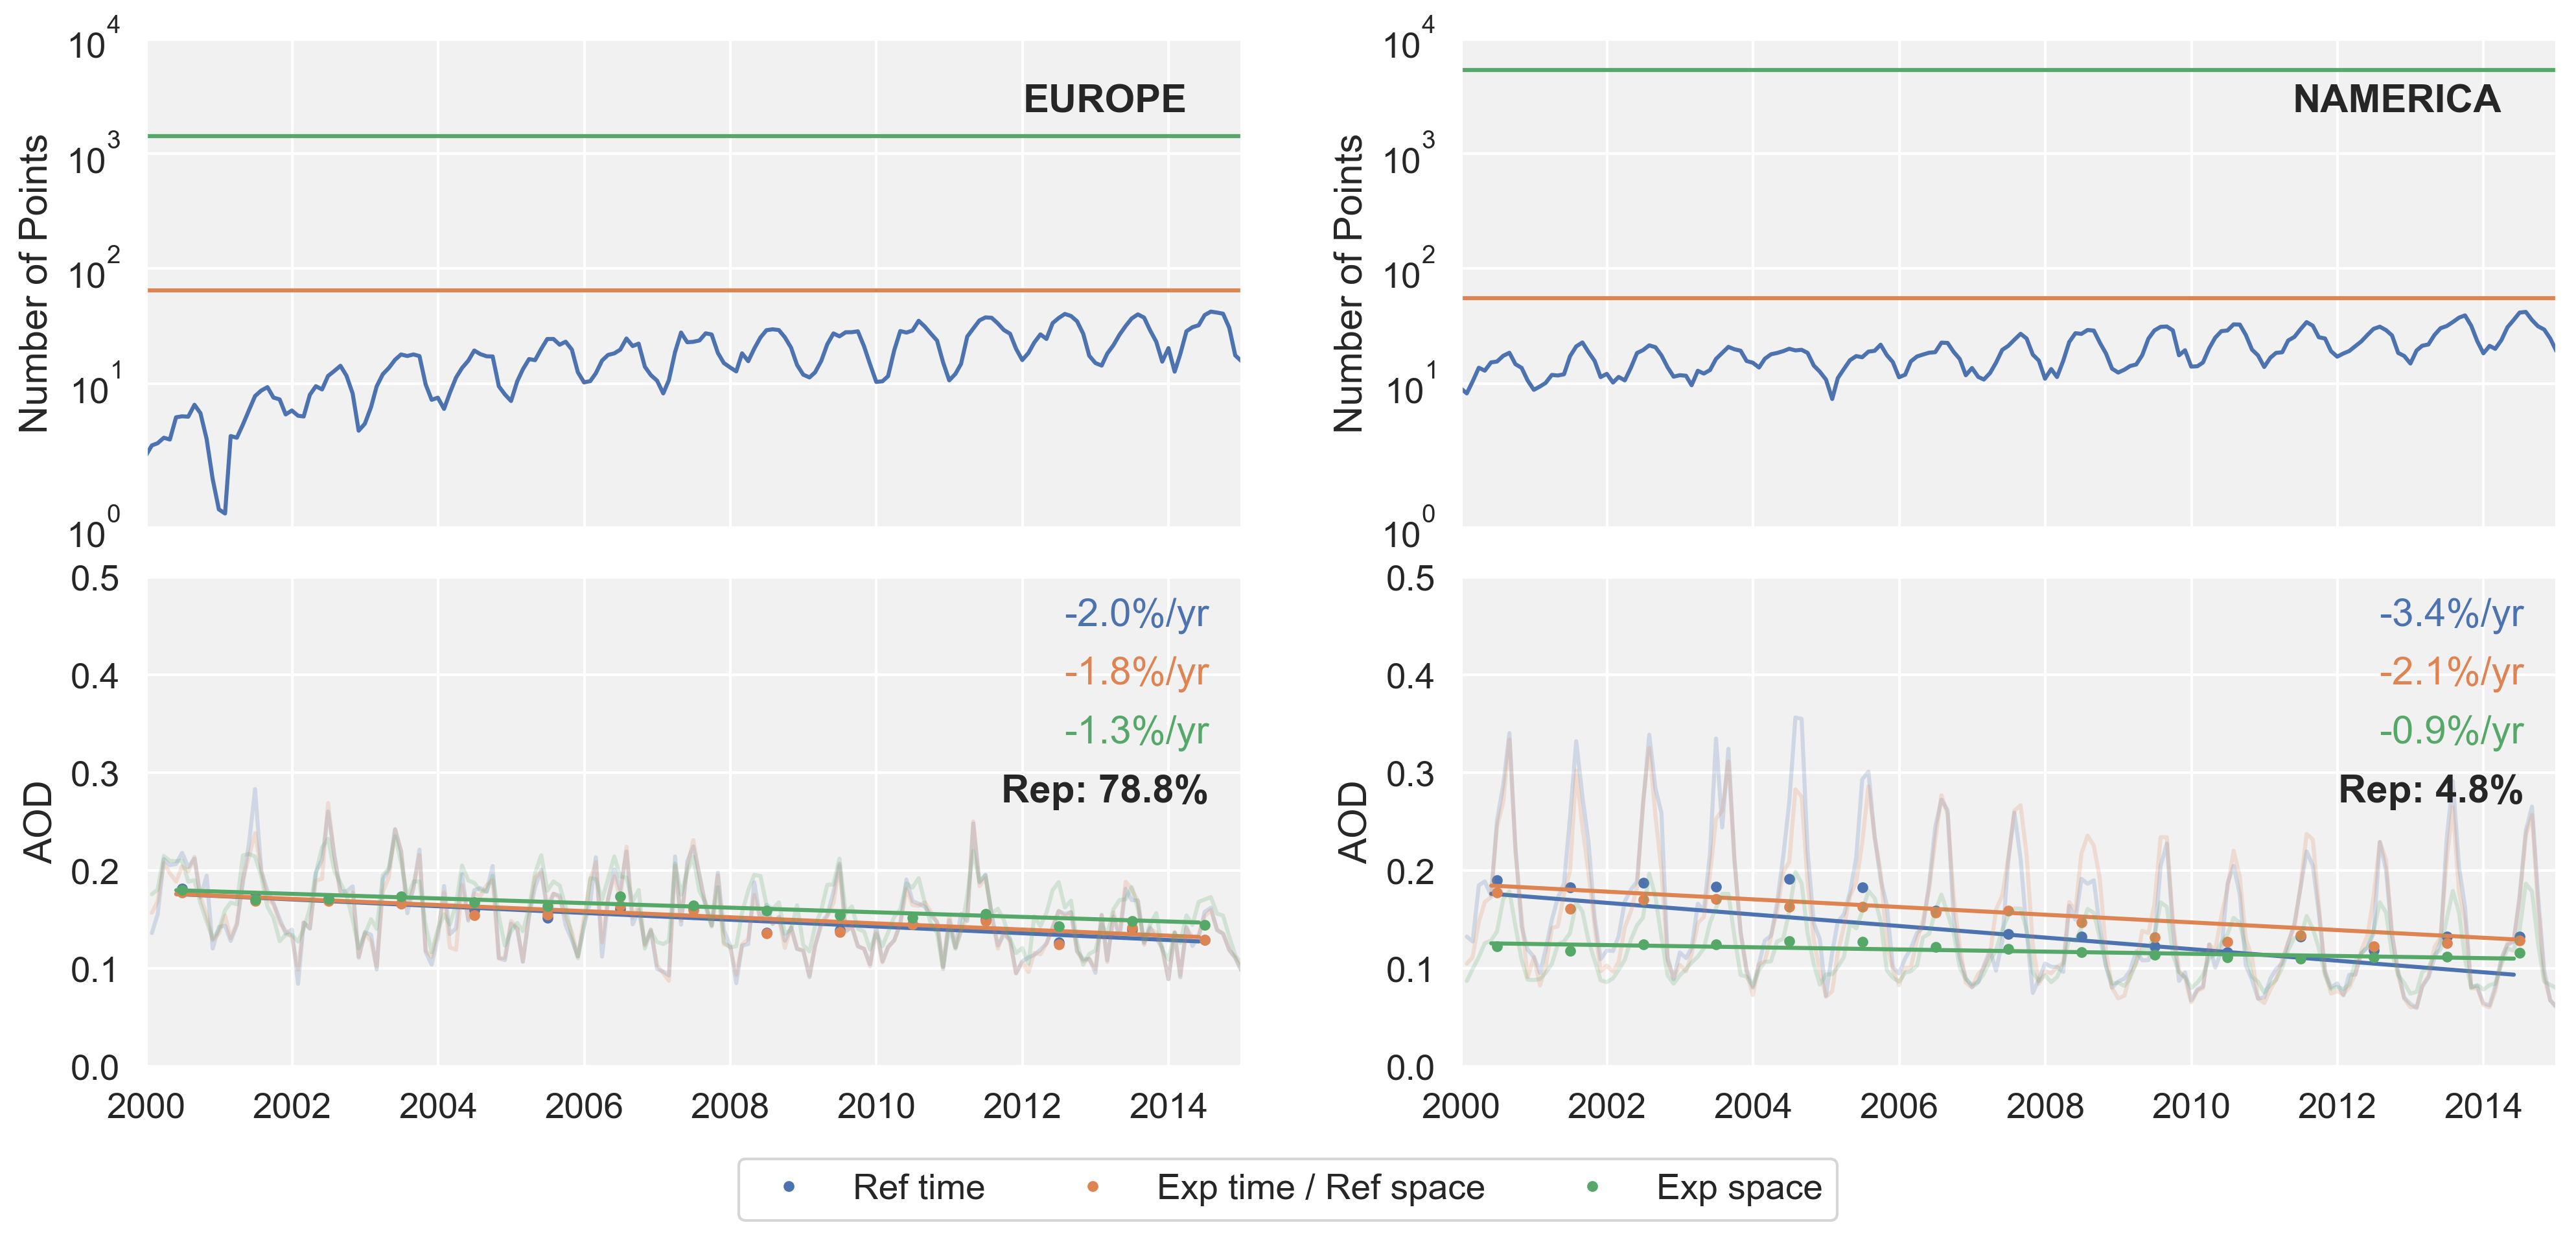
\includegraphics[width=16cm]{../scripts/figs/representativity.png}
 \caption{Representativity of the regional AOD time series for the computation of trends. The upper figures correspond to the number of points used to compute the regional time series. The lower figures show the time series, the trends, and the resulting representativity.}
 \label{fig:representativity}
\end{figure}

\appendixfigures  %% needs to be added in front of appendix figures

\appendixtables   %% needs to be added in front of appendix tables

%% Please add \clearpage between each table and/or figure. Further guidelines on figures and tables can be found below.



\authorcontribution{TEXT} %% this section is mandatory

\competinginterests{TEXT} %% this section is mandatory even if you declare that no competing interests are present

\disclaimer{TEXT} %% optional section

\begin{acknowledgements}
 TEXT
\end{acknowledgements}




%% REFERENCES

%% The reference list is compiled as follows:

%\begin{thebibliography}{}

% \bibitem[AUTHOR(YEAR)]{LABEL1}
% REFERENCE 1

% \bibitem[AUTHOR(YEAR)]{LABEL2}
% REFERENCE 2

%\end{thebibliography}

%% Since the Copernicus LaTeX package includes the BibTeX style file copernicus.bst,
%% authors experienced with BibTeX only have to include the following two lines:
%%
\bibliographystyle{copernicus}
\bibliography{mybib.bib}
%%
%% URLs and DOIs can be entered in your BibTeX file as:
%%
%% URL = {http://www.xyz.org/~jones/idx_g.htm}
%% DOI = {10.5194/xyz}


%% LITERATURE CITATIONS
%%
%% command                        & example result
%% \citet{jones90}|               & Jones et al. (1990)
%% \citep{jones90}|               & (Jones et al., 1990)
%% \citep{jones90,jones93}|       & (Jones et al., 1990, 1993)
%% \citep[p.~32]{jones90}|        & (Jones et al., 1990, p.~32)
%% \citep[e.g.,][]{jones90}|      & (e.g., Jones et al., 1990)
%% \citep[e.g.,][p.~32]{jones90}| & (e.g., Jones et al., 1990, p.~32)
%% \citeauthor{jones90}|          & Jones et al.
%% \citeyear{jones90}|            & 1990



%% FIGURES

%% When figures and tables are placed at the end of the MS (article in one-column style), please add \clearpage
%% between bibliography and first table and/or figure as well as between each table and/or figure.


%% ONE-COLUMN FIGURES

%%f
%\begin{figure}[t]
%\includegraphics[width=12cm]{FILE NAME}
%\caption{TEXT}
%\end{figure}
%
%%% TWO-COLUMN FIGURES
%
%%f
%\begin{figure*}[t]
%\includegraphics[width=16cm]{FILE NAME}
%\caption{TEXT}
%\end{figure*}
%
%
%%% TABLES
%%%
%%% The different columns must be seperated with a & command and should
%%% end with \\ to identify the column brake.
%
%%% ONE-COLUMN TABLE
%
%%t
%\begin{table}[t]
%\caption{TEXT}
%\begin{tabular}{column = lcr}
%\tophline
%
%\middlehline
%
%\bottomhline
%\end{tabular}
%\belowtable{} % Table Footnotes
%\end{table}
%
%%% TWO-COLUMN TABLE
%
%%t
%\begin{table*}[t]
%\caption{TEXT}
%\begin{tabular}{column = lcr}
%\tophline
%
%\middlehline
%
%\bottomhline
%\end{tabular}
%\belowtable{} % Table Footnotes
%\end{table*}
%
%%% LANDSCAPE TABLE
%
%%t
%\begin{sidewaystable*}[t]
%\caption{TEXT}
%\begin{tabular}{column = lcr}
%\tophline
%
%\middlehline
%
%\bottomhline
%\end{tabular}
%\belowtable{} % Table Footnotes
%\end{sidewaystable*}
%
%
%%% MATHEMATICAL EXPRESSIONS
%
%%% All papers typeset by Copernicus Publications follow the math typesetting regulations
%%% given by the IUPAC Green Book (IUPAC: Quantities, Units and Symbols in Physical Chemistry,
%%% 2nd Edn., Blackwell Science, available at: http://old.iupac.org/publications/books/gbook/green_book_2ed.pdf, 1993).
%%%
%%% Physical quantities/variables are typeset in italic font (t for time, T for Temperature)
%%% Indices which are not defined are typeset in italic font (x, y, z, a, b, c)
%%% Items/objects which are defined are typeset in roman font (Car A, Car B)
%%% Descriptions/specifications which are defined by itself are typeset in roman font (abs, rel, ref, tot, net, ice)
%%% Abbreviations from 2 letters are typeset in roman font (RH, LAI)
%%% Vectors are identified in bold italic font using \vec{x}
%%% Matrices are identified in bold roman font
%%% Multiplication signs are typeset using the LaTeX commands \times (for vector products, grids, and exponential notations) or \cdot
%%% The character * should not be applied as mutliplication sign
%
%
%%% EQUATIONS
%
%%% Single-row equation
%
%\begin{equation}
%
%\end{equation}
%
%%% Multiline equation
%
%\begin{align}
%& 3 + 5 = 8\\
%& 3 + 5 = 8\\
%& 3 + 5 = 8
%\end{align}
%
%
%%% MATRICES
%
%\begin{matrix}
%x & y & z\\
%x & y & z\\
%x & y & z\\
%\end{matrix}
%
%
%%% ALGORITHM
%
%\begin{algorithm}
%\caption{...}
%\label{a1}
%\begin{algorithmic}
%...
%\end{algorithmic}
%\end{algorithm}
%
%
%%% CHEMICAL FORMULAS AND REACTIONS
%
%%% For formulas embedded in the text, please use \chem{}
%
%%% The reaction environment creates labels including the letter R, i.e. (R1), (R2), etc.
%
%\begin{reaction}
%%% \rightarrow should be used for normal (one-way) chemical reactions
%%% \rightleftharpoons should be used for equilibria
%%% \leftrightarrow should be used for resonance structures
%\end{reaction}
%
%
%%% PHYSICAL UNITS
%%%
%%% Please use \unit{} and apply the exponential notation


\end{document}
